\section{Results for Study 1}\label{ch4:study1} 

In this section, we present the results with respect to the \textit{concrete
integration time} dimension. This dimension involves the investigation of
integration time in terms of number of releases and number of days
(\hyperref[def:1]{Definitions}~\ref{def:1} and \ref{def:2}). This dimension is
comprised of \hyperref[ch4:rq1]{RQ1}-\hyperref[ch4:rq4]{RQ4}. Below, we present the
obtained results for each RQ. 
%here goes RQ1, RQ2, and RQ3

\subsection*{\textit{\textbf{RQ1: How often are addressed issues prevented from being
released?}}}\label{resutls:rq1}

\begin{figure}[!t]
	\centering
	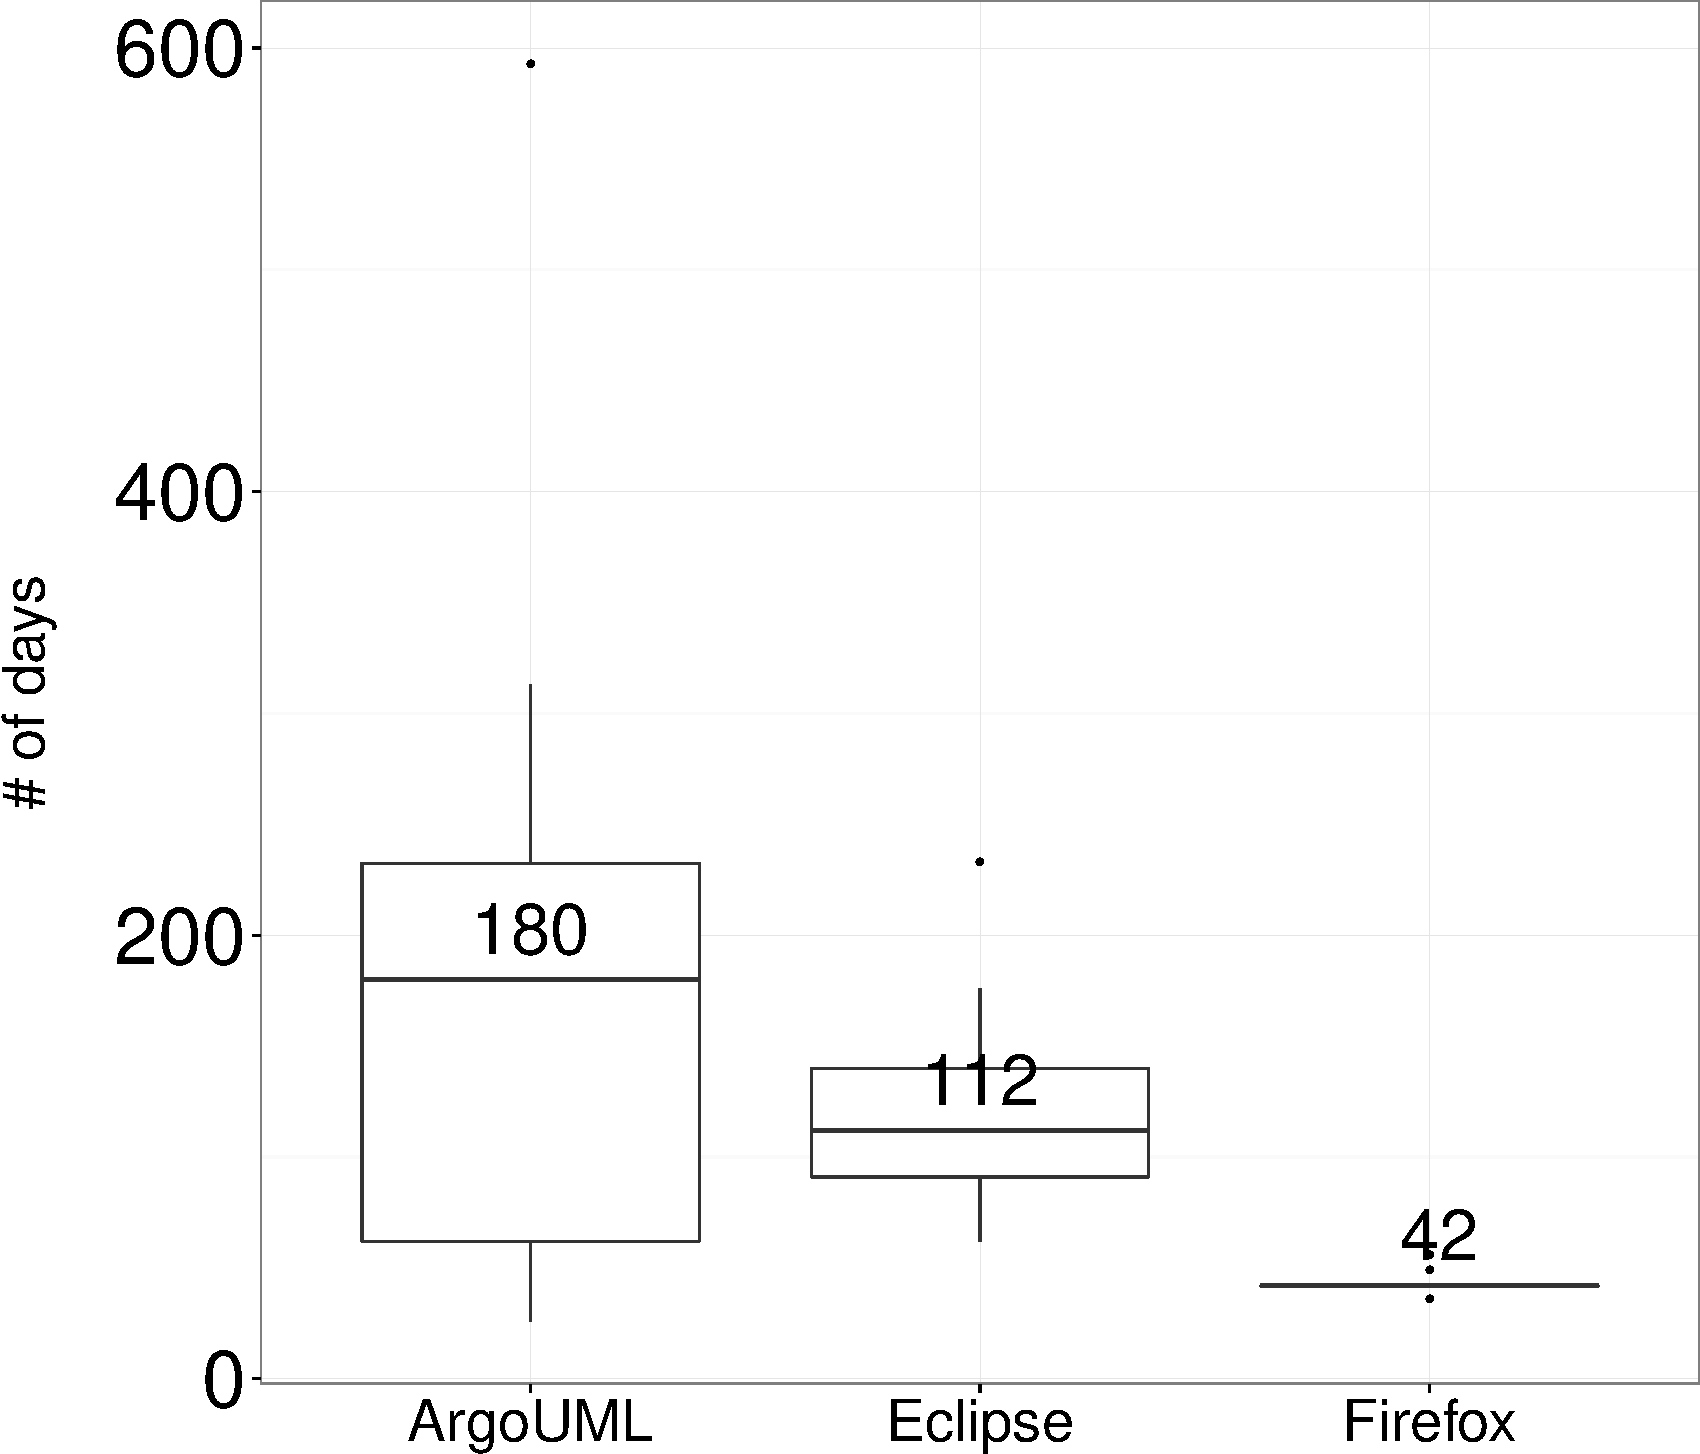
\includegraphics[width=0.7\textwidth]
	{chapters/chapter4/figures/RQ1_time_between_releases.pdf}
	\caption{\textbf{Number of days between the studied releases of the
	ArgoUML, Eclipse, and Firefox projects.} The number shown over each
boxplot is the median interval.}  
	\label{ch4:fig:releaseIntervals}
\end{figure}

\noindent\textit{\textbf{Addressed issues usually
miss the next release in the Firefox project.}}
\hyperref[ch4:fig:releaseIntervals]{Figure}~\ref{ch4:fig:releaseIntervals} shows the
difference between the studied projects in terms of the time interval between
their releases. The median time in days for the Firefox project (42 days) is
approximately $\frac{1}{4}$ that of the ArgoUML project (180 days), and
$\frac{1}{3}$ that of the Eclipse project (112 days). Unlike the Eclipse and
Firefox projects, the distribution for the ArgoUML project is skewed. In
addition, \hyperref[ch4:fig:fixToIntegration]{Figure}~\ref{ch4:fig:fixToIntegration}
shows that the vast majority of addressed issues for the Firefox project is integrated
\textit{after-2} releases, whereas for the Eclipse and ArgoUML projects, the
majority is integrated in the \textit{next} release. 

The reason for the difference may be due to the release policies that are
followed in each project. For example,
\hyperref[ch4:fig:releaseIntervals]{Figure}~\ref{ch4:fig:releaseIntervals} shows that
the Firefox project releases consistently every 42 days (six weeks), whereas the
time intervals between the releases of the ArgoUML project vary from 50 to 220
days. Indeed, the release guidelines for the ArgoUML project state that the
ArgoUML team should release at least one stable release every 8 months (see
\hyperref[argouml:releng]{Section}~\ref{argouml:releng}). The delivery
consistency of the Firefox releases might lead to addressed issues being prevented
from a greater number of releases, since the Firefox project rigidly adhere to a
six-week release schedule despite accumulating issues that could not be
integrated (see \hyperref[firefox:releng]{Section}~\ref{firefox:releng}). 

Although an addressed issue usually misses the next release in the Firefox
project, issues are usually shipped faster when compared to the other projects.
Indeed, \hyperref[ch4:fig:beanplot_days]{Figure}~\ref{ch4:fig:beanplot_days} shows that
addressed issues in the Firefox project take a median of 107 days to be
released, while it takes 166 and 146 days in the Eclipse and ArgoUML projects,
respectively.\\

\noindent\textit{\textbf{34\% to 60\% of addressed issues had their integration
prevented from at least one release in the traditionally released projects.}}
\hyperref[ch4:fig:fixToIntegration]{Figure}~\ref{ch4:fig:fixToIntegration} shows that
98\% of the addressed issues in the Firefox project are prevented from integration
in at least one release. However, for the projects that adopt a more traditional
release cycle, \ie the ArgoUML and Eclipse projects, 34\% to 60\%  of the addressed
issues are prevented from integration in at least one release. This result
indicates that even though an issue is addressed, integration may be prevented by
one or more releases, which can frustrate end users.\\

\begin{figure}[!t]
	\centering
	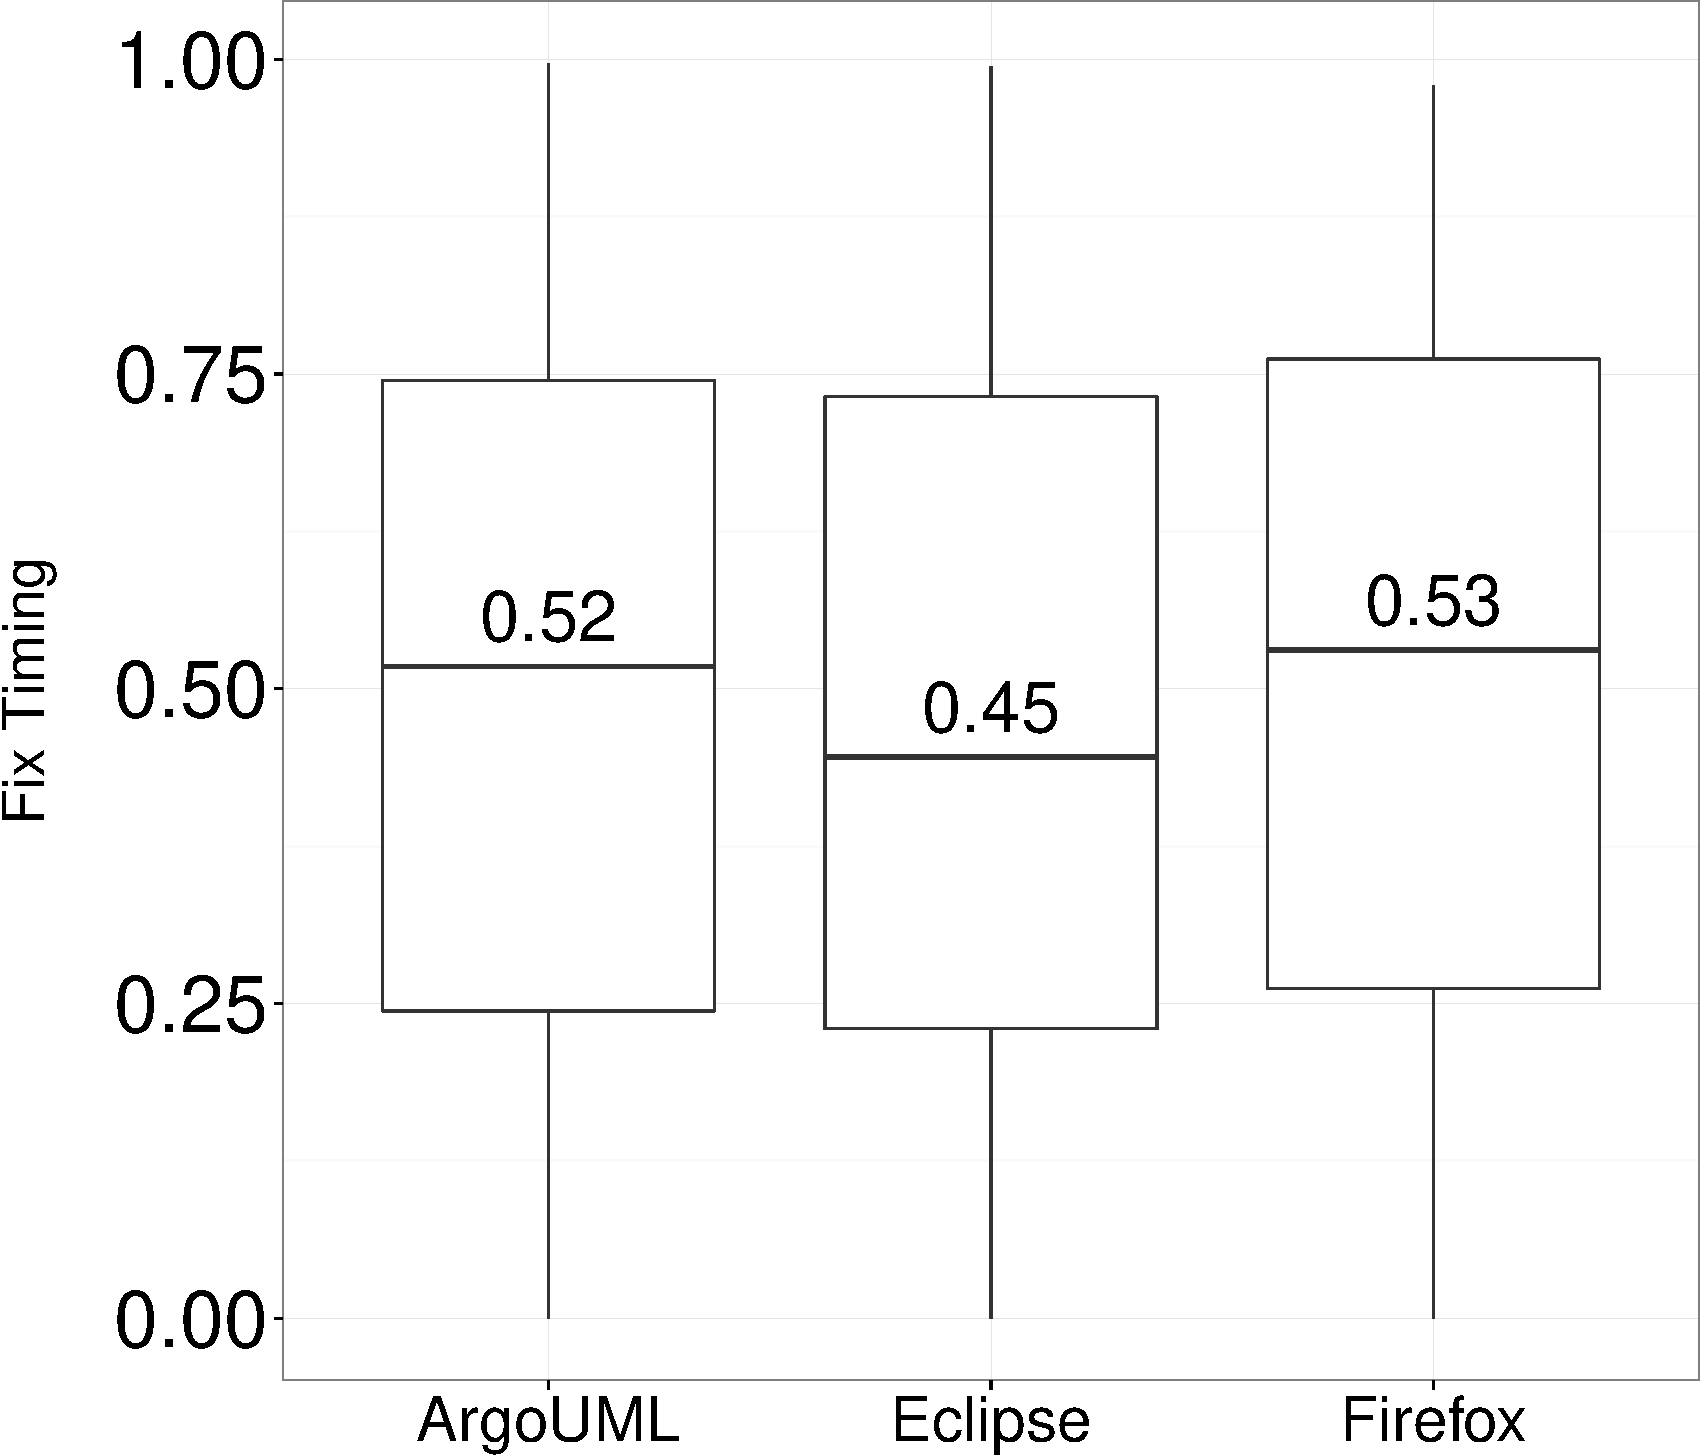
\includegraphics[width=0.7\textwidth]
	{chapters/chapter4/figures/addressing_stage.pdf}
	\caption{\textbf{Fix timing metric.} We present the
		distribution of the \textit{fix timing} metric for addressed
		issues that are prevented from integration in at least one release.}
	\label{ch4:fig:boxplotTimeWindow}
\end{figure}

\noindent\textit{\textbf{Many issues that were prevented from integration are
addressed well before the upcoming release date.}} addressed issues could be prevented
from integration because they were addressed late in the release cycle, \eg one day
or one week before the upcoming release date. To check whether addressed issues are
being prevented from integration mostly because they are being addressed late in the
release cycle, we compute the \textit{fix timing} metric. 

\hyperref[ch4:fig:boxplotTimeWindow]{Figure}~\ref{ch4:fig:boxplotTimeWindow} shows the
distribution of the \textit{fix timing} metric for each project. The smallest
\textit{fix timing} median is observed for the Eclipse project, which is 0.45.
For the ArgoUML and Firefox projects, the median is 0.52 and 0.53, respectively.
The \textit{fix timing} medians are roughly in the middle of the release.
Moreover, the boxes extend to cover between 0.25 and 0.75. The result suggests
that, in the studied projects, issues that are prevented from integration are
usually addressed $\frac{1}{4}$ to $\frac{3}{4}$ of the way through a release.
Hence, it is unlikely that most addressed issues are prevented from integration
solely because they were addressed too close to an upcoming release date.

\conclusionbox{The integration of 34\% to 60\% of the addressed issues in the
	traditionally released projects and 98\% in the rapidly released project
	were prevented from integration in at least one release. Furthermore, we
	find that many issues which integration was prevented, were addressed well
before the releases from which they were omitted.}


\subsection*{\textbf{\textit{RQ2: Does the stage of the release cycle impact delivery delay?}}}

\noindent\textit{\textbf{Issues that are addressed during more stable stages of a
release cycle have a shorter delivery delay.}}
\hyperref[ch4:fig:cycle_phases]{Figure}~\ref{ch4:fig:cycle_phases} shows the
distributions of delivery delay (in terms of days) per each release cycle
stage of the studied projects. For the Eclipse project, the stages are divided
into {\em milestones}, {\em RCs} (Release Candidates), and {\em code freeze}
(see the \hyperref[eclipse:releng]{release engineering} process of Eclipse). Indeed, issues that
are addressed during RCs have a shorter delivery delay when
compared to issues that were addressed during milestone releases. For the difference
between {\em milestones} and {\em RCs}, we observe a $p=1.47 \times 10^{-52}$ and a {\em
large} effect-size of $delta=0.63$. All of the $p$-$values$ and $deltas$ of our
statistical analysis are shown in
\hyperref[ch4:tbl:statisticalrq2]{Table}~\ref{ch4:tbl:statisticalrq2}. Even though
delivery delay seems to be larger during the {\em code freeze} stage, we do
not observe a significant $p$-$value$ when comparing the {\em code freeze} stage
to the other stages. In fact, only ten issues were addressed during the {\em code freeze}
stage in our data, which impairs statistical observations of trends in such a stage.

For the Firefox project, we observe that delivery delay tends to be
shorter as fixes are performed along more stable stages. For example, by
comparing the delivery delay values between the {\em NIGHTLY} and {\em
AURORA} stages, we observe a $p=5.1 \times 10^{-49}$ and a {\em medium}
effect-size of $delta = 0.40$ (the other comparisons are shown in
\hyperref[ch4:tbl:statisticalrq2]{Table}~\ref{ch4:tbl:statisticalrq2}).

Finally, for the ArgoUML project, we also observe a trend of shorter
delivery delay as the fixes are performed during more stable stages of release
cycles. For instance, when we compare the delivery delay of addressed issues of the {\em alpha}
and {\em beta} stages, we obtain a $p$-$value$ of $3.98 \times 10^{-09}$ and a {\em
large} effect-size of $delta = 0.98$.\\

\begin{figure}
	\centering
	\subfloat[Eclipse]{
		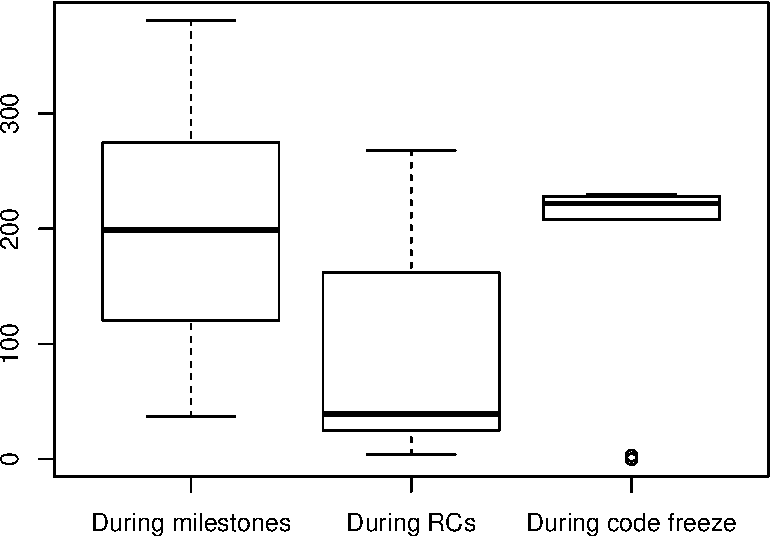
\includegraphics[width=0.60\textwidth,keepaspectratio]
		{chapters/chapter4/figures/eclipse_phases_boxplot.pdf}
	}

	\subfloat[Firefox]{
		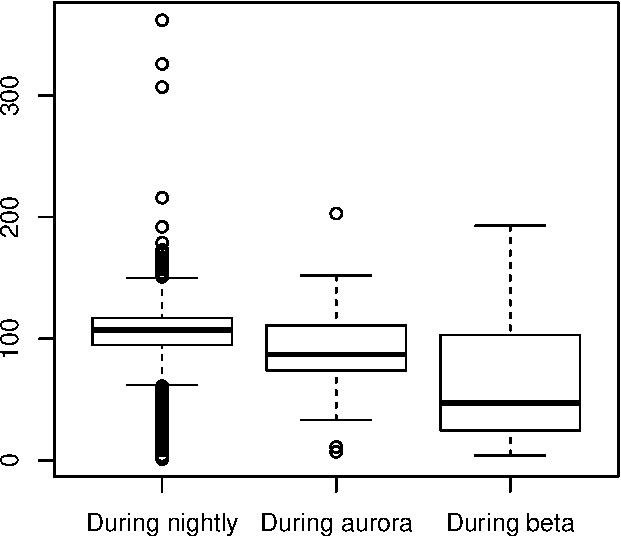
\includegraphics[width=0.60\textwidth,keepaspectratio]
		{chapters/chapter4/figures/firefox_phases_boxplot.pdf}
	}

	\subfloat[ArgoUML]{
		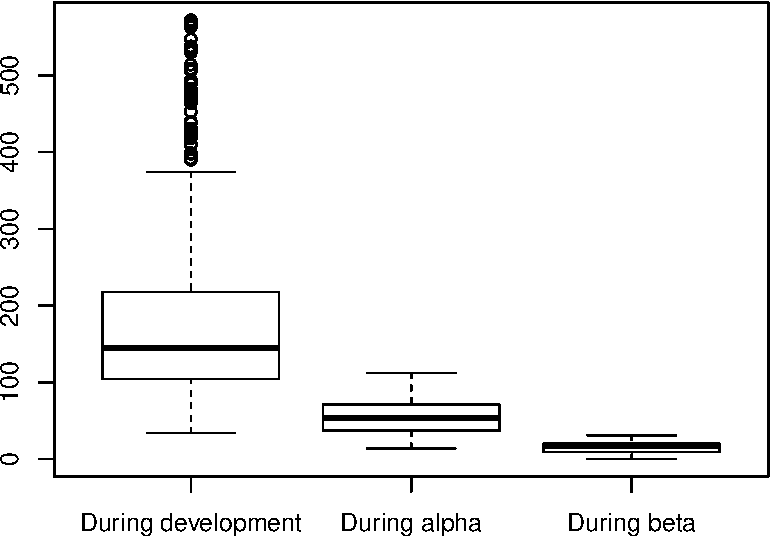
\includegraphics[width=0.60\textwidth,keepaspectratio]
		{chapters/chapter4/figures/argouml_phases_boxplot.pdf}
	}

	\caption{\textbf{delivery delay during release
		cycle stages.} Issues that are addressed during more stable stages of a release cycle
	are likely to have a shorter delivery delay}
	\label{ch4:fig:cycle_phases}
\end{figure}


\begin{table}
	\footnotesize
	\centering
	\caption{\textbf{Statistical analysis.} An overview of the $p$-$values$
		and $deltas$ that are observed during our statistical analyses.
		\label{ch4:tbl:statisticalrq2}
	}
	\resizebox{\textwidth}{!}{
		\begin{tabular}{llrrr}
			\hline 
			& \textbf{Comparison} & \textbf{Kruskal-Wallis} ($p$) &
			\textbf{Dunn} ($p.adjusted$) & \textbf{Effect-size} ($delta$)\tabularnewline
			\hline 
			\multirow{3}{*}{\textbf{Eclipse}} & Milestones vs RCs &
			\multirow{3}{*}{$1.87 \times 10^{-51}$} & $1.47 \times 10^{-52}$ & (large) $0.63$\tabularnewline
			\cline{2-2} \cline{4-5} & RCs vs Code freeze &  & $0.56$ & Not apply\tabularnewline \cline{2-2} \cline{4-5} & Milestones vs Code freeze &  & $0.02$ & (negligible) $0.09$\tabularnewline
			\hline 
			\multirow{3}{*}{\textbf{Firefox}} & Nightly vs Aurora &
			\multirow{3}{*}{$2.99 \times 10^{-76}$} & $5.07 \times 10^{-49}$ &
			(medium) $0.40$\tabularnewline
			\cline{2-2} \cline{4-5} 
			& Aurora vs Beta &  & $1.72 \times 10^{-03}$ & (medium) $0.40$\tabularnewline
			\cline{2-2} \cline{4-5} 
			& Nightly vs Beta &  & $1.43 \times 10^{-31}$ & (large) $0.57$\tabularnewline
			\hline 
			\multirow{3}{*}{\textbf{ArgoUML}} & Development vs Alpha
			& \multirow{3}{*}{$2.73 \times 10^{-135}$} & $7.24 \times 10^{-89}$
			& (large) $0.94$\tabularnewline
			\cline{2-2} \cline{4-5} 
			& Alpha vs Beta &  & $3.98 \times 10^{-09}$ & (large) $0.98$\tabularnewline
			\cline{2-2} \cline{4-5} 
			& Development vs Beta &  & $1.14 \times 10^{-78}$ & (large) $0.99$\tabularnewline
			\hline 
		\end{tabular}
	}
\end{table}

\noindent\textit{\textbf{Many issues that are prevented from integration are
addressed well before the code freeze stage of their respective release cycle.}} We
compute the {\em fix timing} metric that we present in \hyperref[rq1]{RQ1}.
However, instead of counting the number of days until an upcoming release, we
count the number of days until an upcoming code freeze stage
(\hyperref[ch4:eq:fixtiming2]{Equation}~\ref{ch4:eq:fixtiming2}). Our goal is to check
whether addressed issues are being prevented from integration mostly because they
are being addressed too close to a code freeze stage (\ie a period during which
integration of new code changes would likely be minimal).  

\begin{figure} \center 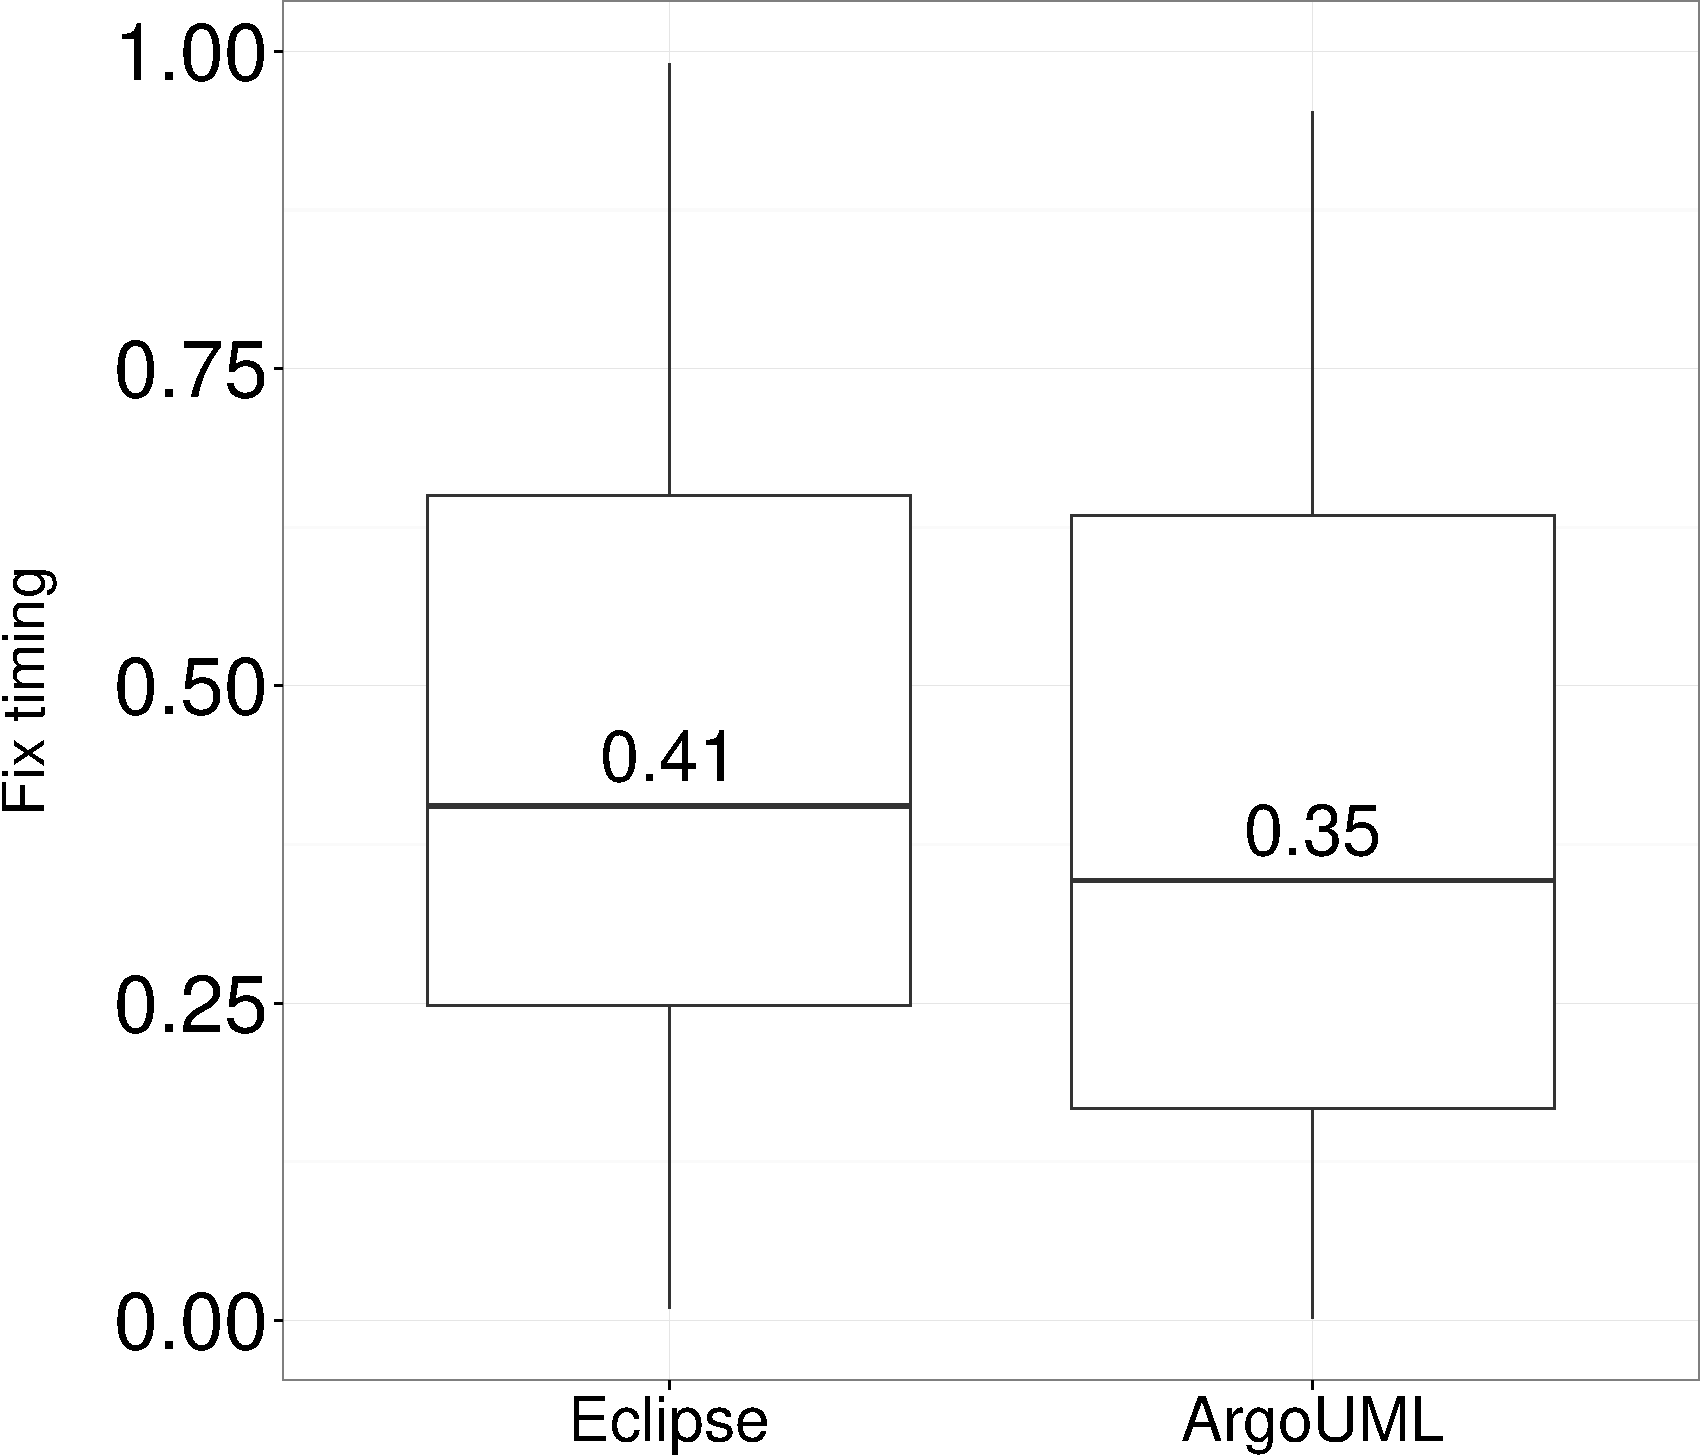
\includegraphics[width=0.60\textwidth,keepaspectratio]
	{chapters/chapter4/figures/as_codefreeze.pdf} \caption{\textbf{{\em Fix timing} values for
		the code freeze period.} The median {\em fix timing} values drop
		from 0.45 and 0.52 to 0.41 and 0.35 in the Eclipse and ArgoUML
projects, respectively. } \label{ch4:fig:codefreeze_allsystems} \end{figure}

In \hyperref[ch4:fig:codefreeze_allsystems]{Figure}~\ref{ch4:fig:codefreeze_allsystems},
we show the {\em fix timing} values for the Eclipse and ArgoUML projects, since
both projects adopt a {\em code freeze} stage. For the Eclipse project, the code
freeze starts after the last release candidate, while for the ArgoUML project,
the code freeze starts at the beginning of the {\em beta} stage (see
\hyperref[ch4:sec:subjects]{Section}~\ref{ch4:sec:subjects}). Naturally, we observe a
drop in the {\em fix timing} values, since both code freeze stages start considerably
before the official release dates. Nevertheless, we observe that even after correcting for
the code freeze stages of the Eclipse and ArgoUML projects, it is unlikely
that addressed issues are being prevented from integration solely because of an approaching code
freeze stage. For instance, although the median {\em fix timing} for the ArgoUML project
dropped from 0.52 to 0.35, the development team would still have 2 months to
integrate an addressed issue---since the median duration of a release cycle in the
ArgoUML project is 180 days.

\conclusionbox{We observe that issues that are addressed during more stable stages of
release cycles are associated with a shorter delivery delay. We also observe
that addressed issues are unlikely to be prevented from integration solely because
they were addressed near an upcoming code freeze stage.}


\subsection*{\textbf{\textit{RQ3: How well can we model the delivery delay of addressed issues?}}}

\begin{figure}
	\centering
	%\captionsetup{justification=centering}
	\subfloat[Eclipse]{
		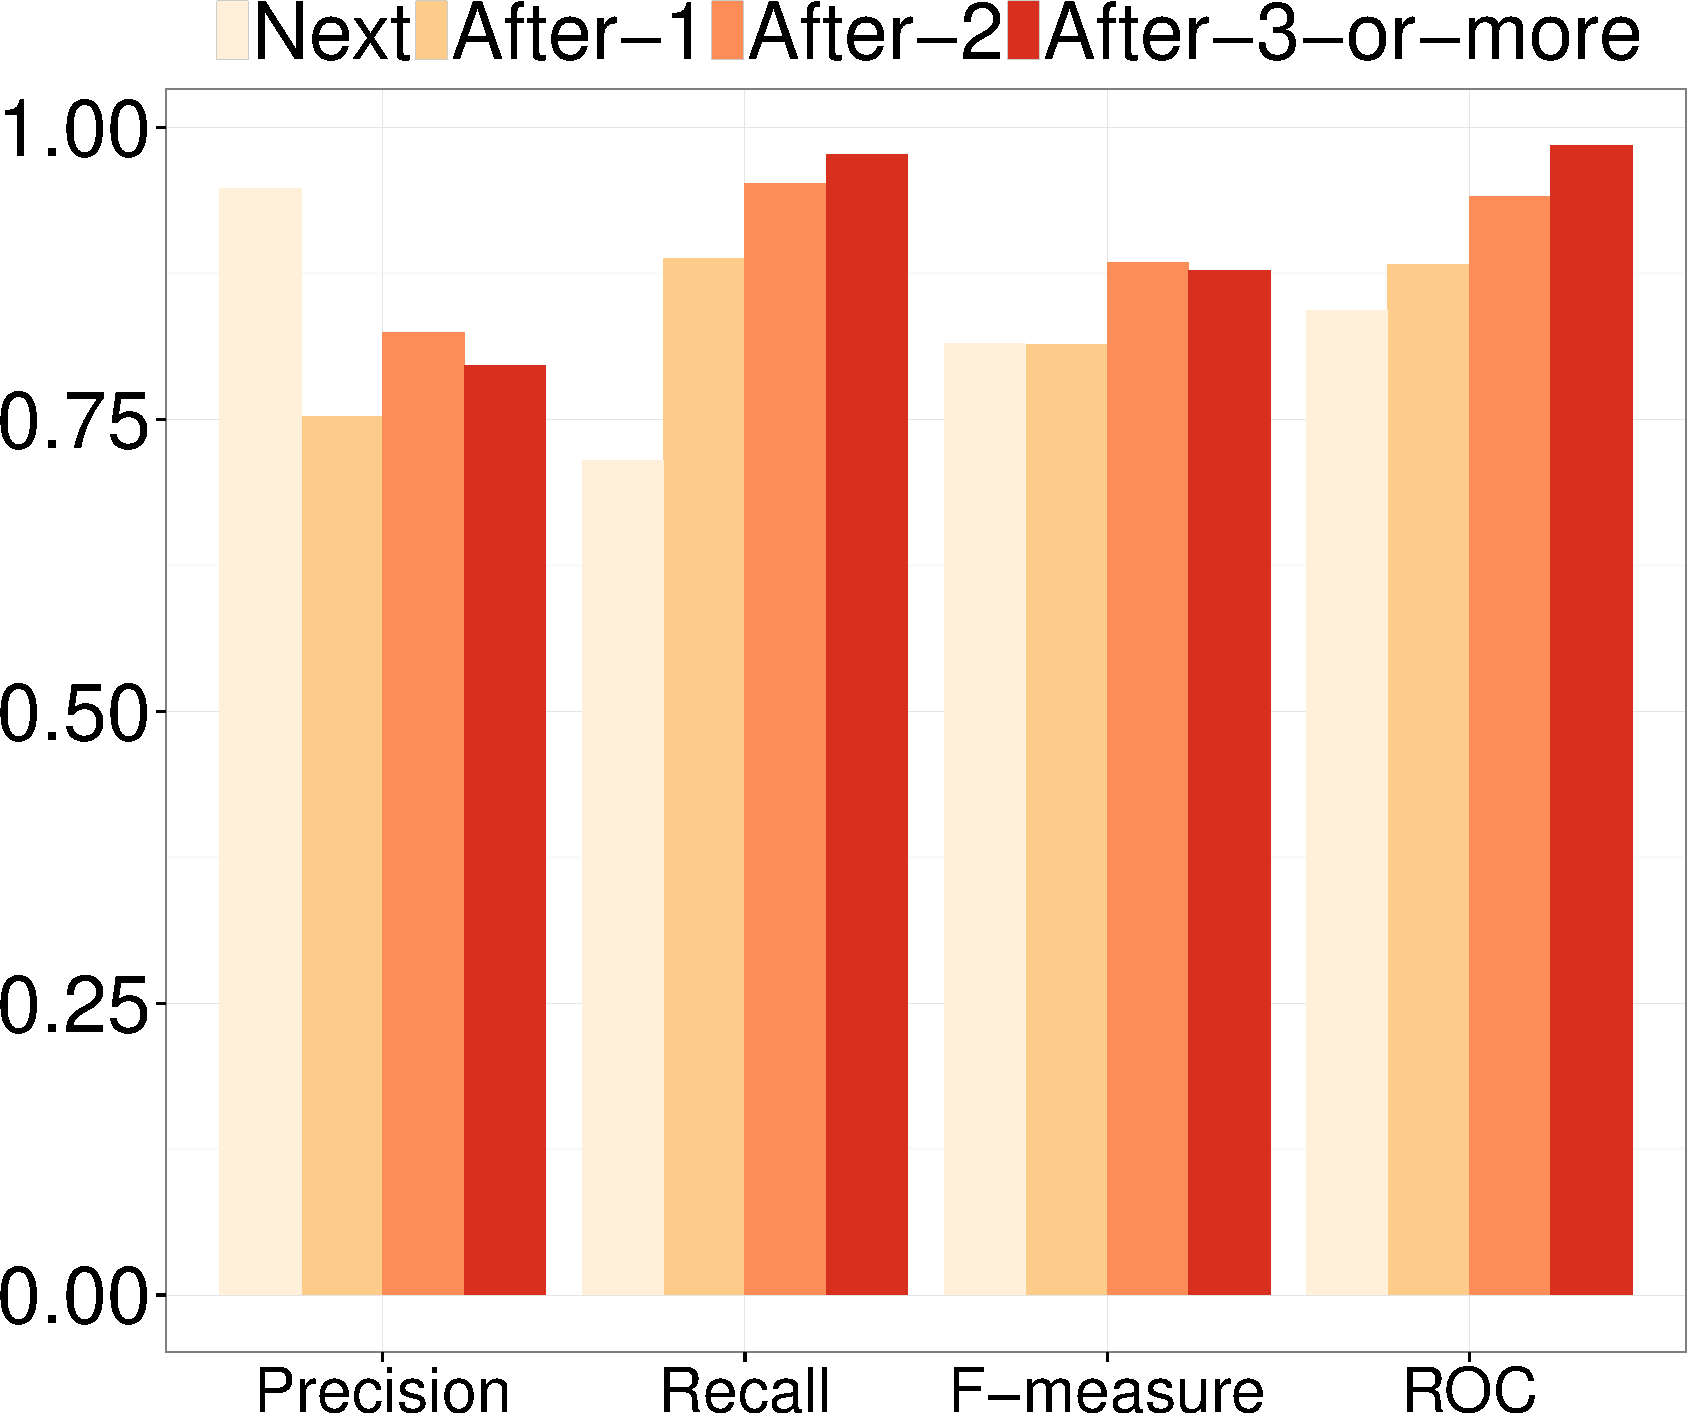
\includegraphics[width=0.50\textwidth,keepaspectratio] 
		{chapters/chapter4/figures/eclipse_loocv_evaluation.pdf}
		\label{ch4:fig:RFeclipse}
	}

	\subfloat[Firefox]{
		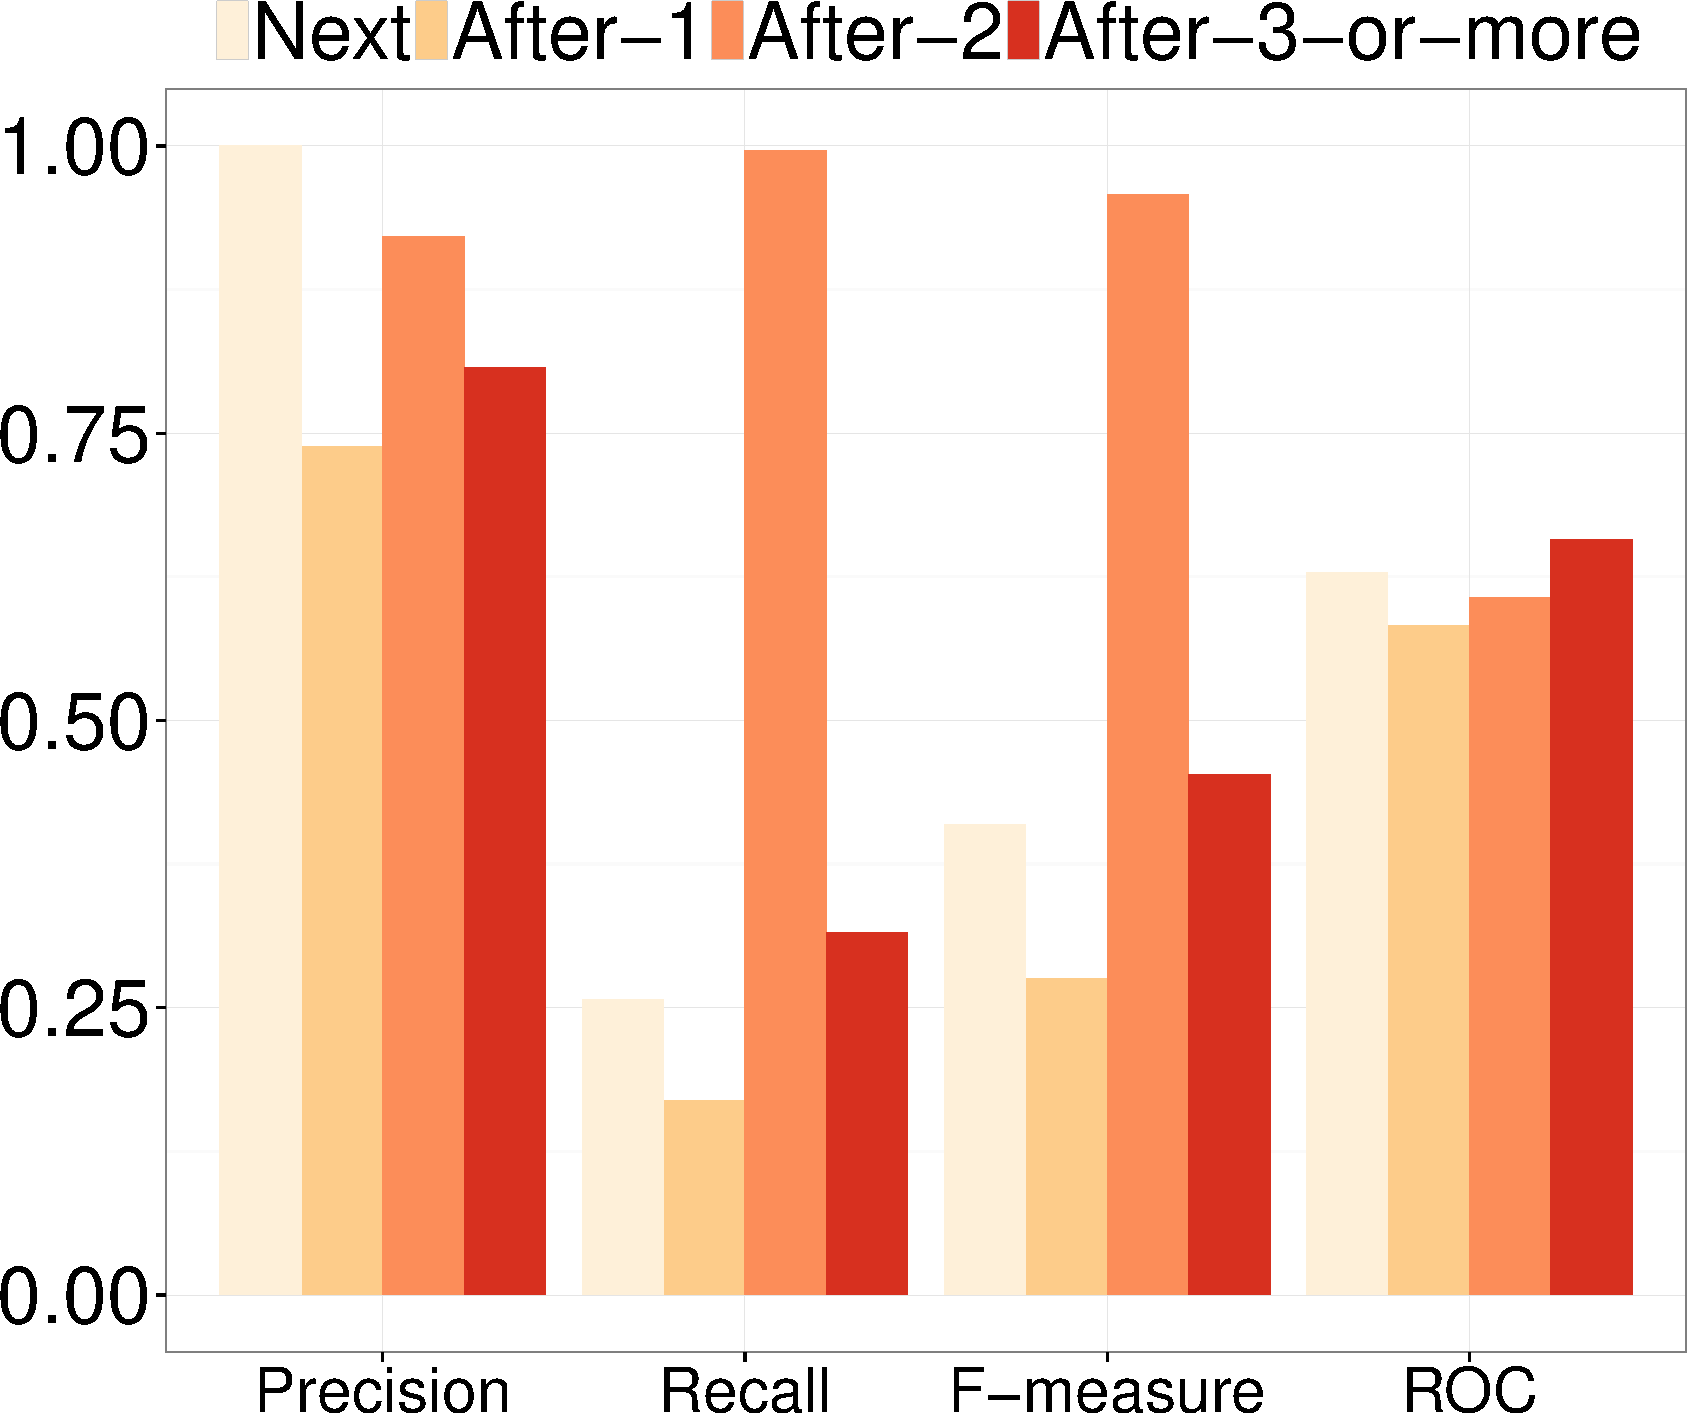
\includegraphics[width=0.50\textwidth,keepaspectratio]  
		{chapters/chapter4/figures/firefox_loocv_evaluation.pdf}
		\label{ch4:fig:RFfirefox}
	}

	\subfloat[ArgoUML]{
		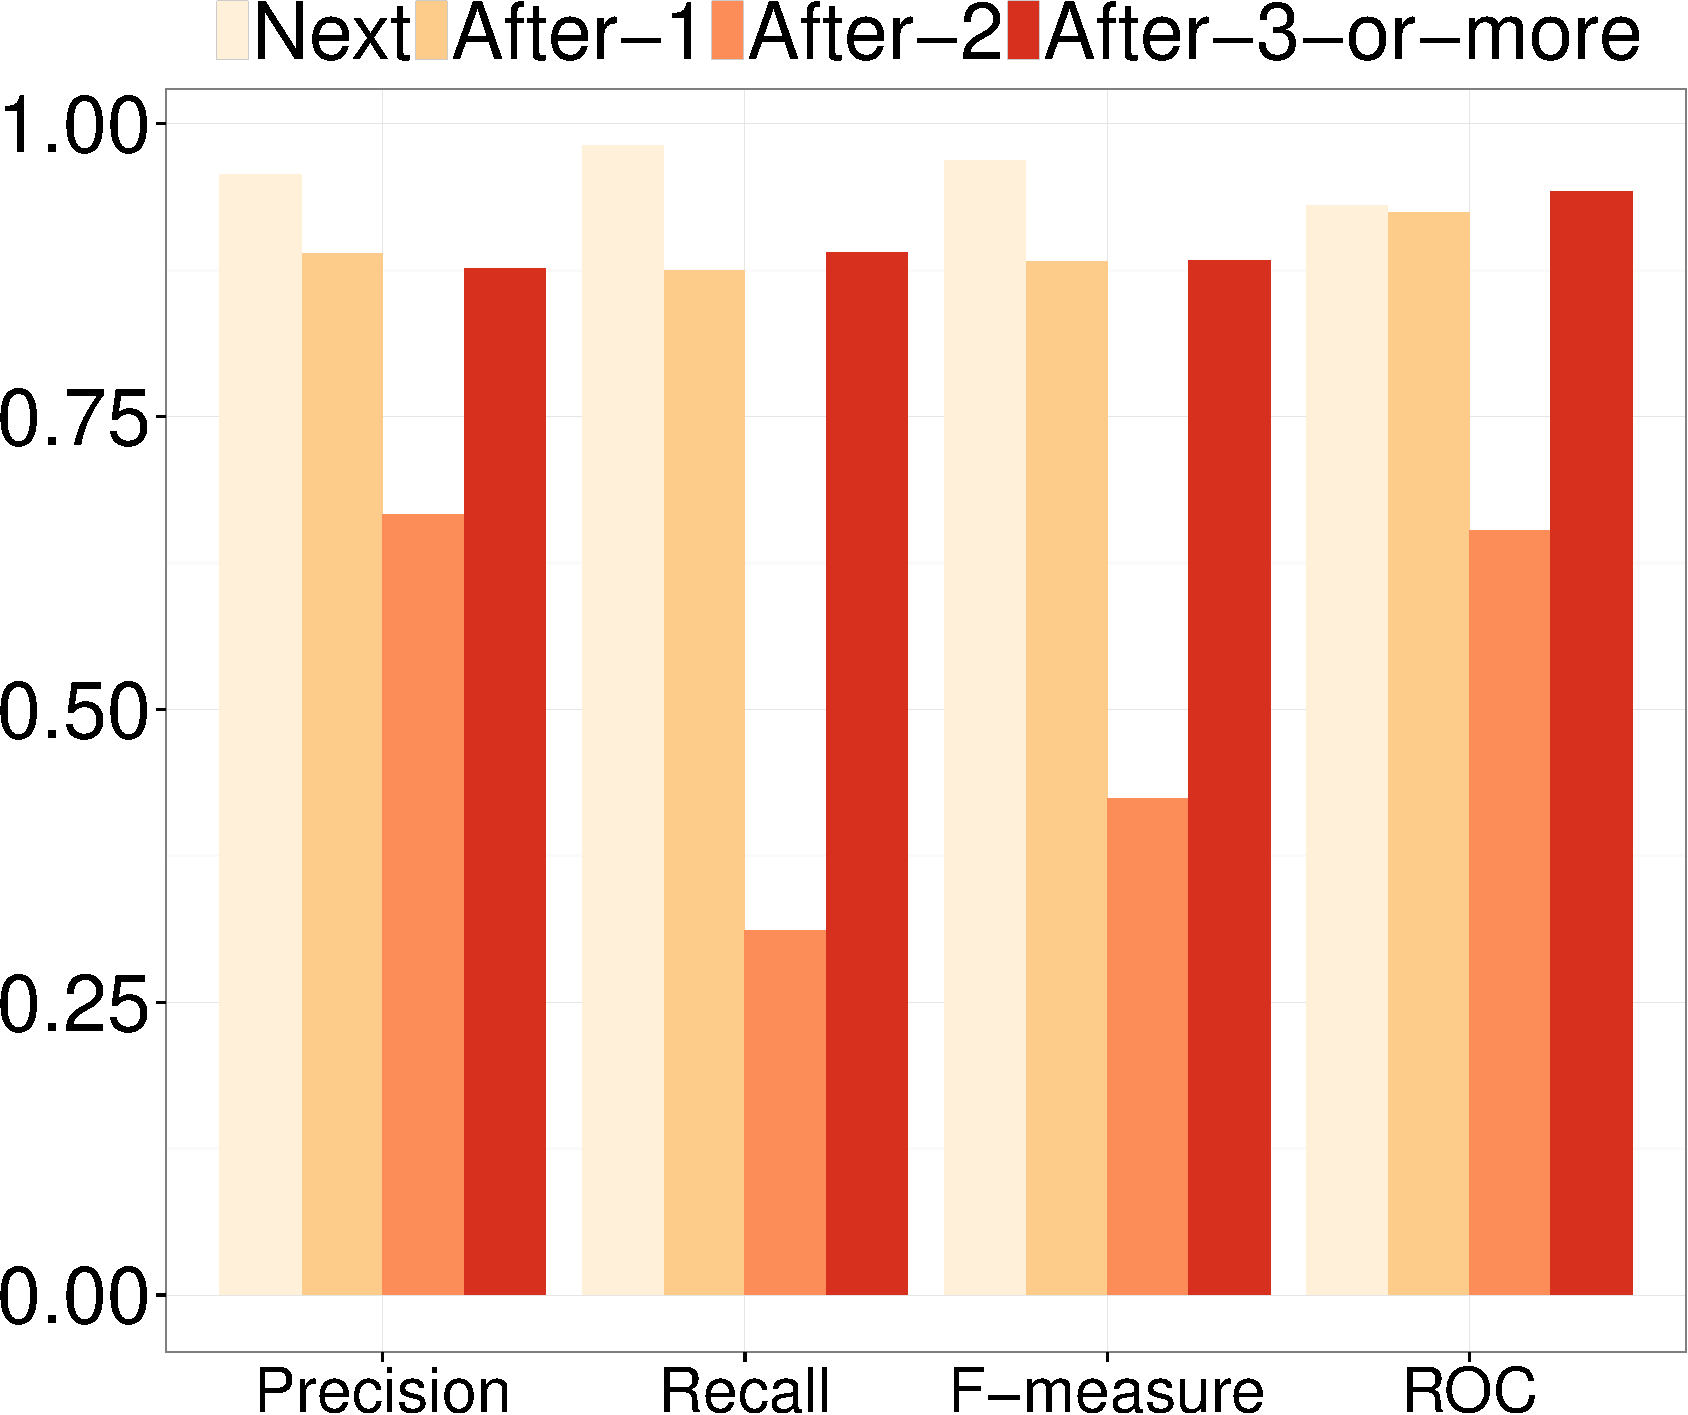
\includegraphics[width=0.50\textwidth,keepaspectratio] 
		{chapters/chapter4/figures/argouml_loocv_evaluation.pdf}
		\label{ch4:fig:RFargo}
	}
	\caption{\textbf{Performance of random forest models.} We show the
	values of Precision, Recall, F-measure, and AUC that are
computed using the LOOCV technique.}
	\label{ch4:fig:RFclassificationResult}
\end{figure}

\begin{table}
	\footnotesize
	\centering
	\caption{The precision, recall, F-measure, and AUC values that are
	obtained for the Eclipse, Firefox, and ArgoUML projects. 
	\label{ch4:tbl:evaluation_metrics}
	}
	\begin{tabular}{lcccc}
		\hline
		\multicolumn{5}{c}{\textbf{Eclipse}}\tabularnewline
		\hline 
		\textbf{Bucket} & \textbf{Precision} & \textbf{Recall} &
		\textbf{F-measure} & \textbf{AUC}\tabularnewline
		\hline 
		Next & 0.95  & 0.71  & 0.81 & 0.84 \tabularnewline
		\hline 
		After-1 & 0.75 & 0.89 & 0.81 & 0.88\tabularnewline
		\hline 
		After-2 & 0.82 & 0.95 & 0.88 & 0.94\tabularnewline
		\hline 
		After-3-or-more & 0.80 & 0.98 & 0.88 & 0.98\tabularnewline
		\hline 
		\hline
		\multicolumn{5}{c}{\textbf{Firefox}}\tabularnewline
		\hline 
		\textbf{Bucket} & \textbf{Precision} & \textbf{Recall} &
		\textbf{F-measure} & \textbf{AUC}\tabularnewline
		\hline 
		Next & 0.99  & 0.26  & 0.41 & 0.63 \tabularnewline
		\hline 
		After-1 & 0.74 & 0.17 & 0.28 & 0.58\tabularnewline
		\hline 
		After-2 & 0.92 & 0.99 & 0.96 & 0.61\tabularnewline
		\hline 
		After-3-or-more & 0.81 & 0.32 & 0.45 & 0.66\tabularnewline
		\hline 
		\hline
		\multicolumn{5}{c}{\textbf{ArgoUML}}\tabularnewline
		\hline 
		\textbf{Bucket} & \textbf{Precision} & \textbf{Recall} &
		\textbf{F-measure} & \textbf{AUC}\tabularnewline
		\hline 
		Next & 0.96  & 0.98  & 0.97 & 0.93 \tabularnewline
		\hline 
		After-1 & 0.89 & 0.87 & 0.88 & 0.92\tabularnewline
		\hline 
		After-2 & 0.67 & 0.31 & 0.42 & 0.65\tabularnewline
		\hline 
		After-3-or-more & 0.88 & 0.89 & 0.88 & 0.94\tabularnewline
		\hline 
	\end{tabular}
\end{table}

\subsubsection*{\textit{\textbf{RQ3: Results for delivery delay in terms of
releases}}}

\noindent\textit{\textbf{Our explanatory models obtain a median precision of 0.81 to
0.88 and a median recall of 0.29 to 0.92.}}
\hyperref[ch4:fig:RFclassificationResult]{Figure}~\ref{ch4:fig:RFclassificationResult}
shows the precision, recall, F-measure, and AUC of our explanatory models.  The
bar charts show the values that we observe for each bucket. The values of
precision, recall, F-measure, and AUC are also shown in
\hyperref[ch4:tbl:evaluation_metrics]{Table}~\ref{ch4:tbl:evaluation_metrics}. 

The best precision/recall values that we obtain for the Eclipse, Firefox, and
ArgoUML projects are related to the \textit{after-2} (F-measure of 0.88),
\textit{after-2} (F-measure of 0.96), and \textit{next} (F-measure of 0.97),
respectively. However, for buckets with low number of instances,
precision/recall values decrease considerably. For instance, the F-measures that
are obtained by our models for the Firefox project are considerably low for the
\textit{next}, \textit{after-1}, and \textit{after-3-or-more} buckets (0.41,
0.28 and 0.45, respectively).

Moreover, our models obtain median AUCs between 0.62 to 0.96, which indicate
that our model estimations are better than random guessing (AUC of 0.5).
Summarizing the results, our models obtain a median precision of 0.81-0.88
(median) and a median recall of 0.29-0.92. Our models provide a sound starting
point for studying the release into which an addressed issue will be integrated.\\

\noindent\textit{\textbf{Our models obtain better F-measure values than
Zero-R.}} We compared our models to Zero-R models as a baseline. For all test
instances, Zero-R selects the bucket that contains the majority of the instances.
Hence, the recall for the bucket containing the majority of instances is 1.0. We
compared the F-measure of our models to the F-measure of Zero-R models. We
choose to compare to the F-measure values because precision and recall are very
skewed for Zero-R. 

For the Firefox project, Zero-R obtains an F-measure of 0.95 for the
\textit{after-2} bucket, whereas our model obtains an F-measure of 0.96 for the
same bucket. For the Eclipse project, Zero-R always selects \textit{next} and
obtains a F-measure of 0.58, while our model obtains an F-measure of 0.81.
Finally, for the ArgoUML project, Zero-R always selects \textit{next} with an
F-measure of 0.84, whereas our model obtains an F-measure of 0.97. These results
show that our models yield better F-measure values than na\"{i}ve techniques
like Zero-R or random guessing (AUC = 0.5) in the majority of cases.  

\conclusionbox{We are able to accurately model how many releases an addressed issue
is likely to be prevented from integration. Our models outperform na\"{i}ve
techniques, such as Zero-R and random guessing, obtaining AUC values of 0.62 to
0.96.}

\begin{table}
	\centering
	\footnotesize
	\caption{\textbf{Regression results of model fit.} Our explanatory
		models obtain $R^2$ values between 0.39 to 0.65 and MAE values between
	7.8 to 66 days.}
	\label{ch4:tbl:regression_results}
	\def\arraystretch{1.5}
	\begin{tabular}{lrrr}
		\hline 
		\centering{\textbf{Metric/Project}} &
		\centering{\textbf{Eclipse}} & \centering{\textbf{Firefox}} &
		\centering{\textbf{ArgoUML}} \tabularnewline
		\hline 
		$R^2$ & 0.48  & 0.39 & 0.65 \tabularnewline
		\hline 
		MAE (days) & 61 & 7.8  & 66 \tabularnewline
		\hline 
		Release cycle duration (median in days) & 112 & 42 & 180 \tabularnewline
		\hline
		Error ratio $(\frac{MAE}{cycle})$ & 0.54  & 0.18  & 0.37 \tabularnewline
		\hline 
		Optimism & 0.0267 & 0.0162 & 0.0035 \tabularnewline
		\hline 
	\end{tabular}
\end{table}

\subsubsection*{\textit{\textbf{RQ3: Results for delivery delay in terms of days}}}

\noindent\textbf{\textit{Our explanatory models obtain $R^2$ values of 0.39-0.65
and MAE values between 7.8 to 67 days.}} Our models obtain fair $R^2$ values to
model the variability of delivery delay in days in the studied projects.
\hyperref[ch4:tbl:regression_results]{Table}~\ref{ch4:tbl:regression_results} shows the
$R^2$ and MAE values that are obtained by each of our regression models. The
$R^2$ values for the Eclipse, Firefox, and ArgoUML projects are of 0.39, 0.48,
and 0.65, respectively. 
Additionally, our regression models can provide fair
estimations of delivery delay in days, specially for the Firefox project. For
instance, the median interval in days between releases of the Firefox project is
42 days
(see~\hyperref[ch4:fig:releaseIntervals]{Figure}~\ref{ch4:fig:releaseIntervals}), while
the MAE value for the Firefox project is 7.8 days, which equates to an error
ratio of 18\% (see
\hyperref[ch4:tbl:regression_results]{Table}~\ref{ch4:tbl:regression_results}).\\

\noindent\textbf{\textit{Our explanatory models obtain a good stability with bootstrap
calculated optimism between 0.0035 to 0.0267 of the $R^2$ values.}} We also
observe that our regression models are stable.
\hyperref[ch4:tbl:regression_results]{Table}~\ref{ch4:tbl:regression_results} shows the
\textit{bootstrap-calculated} optimism of the $R^2$ values of our models. The
optimism for the Eclipse, Firefox and ArgoUML projects are 0.0267, 0.0162, and 0.0035,
respectively. Such results indicate that our explanatory models are unlikely to
be overfitted to our data and that our models are stable enough for us to perform the
statistical inferences that follow. 

\conclusionbox{We are able to accurately estimate the delivery delay in terms
of number of days. Our models obtain fair $R^2$ values of 0.39 to 0.65. Our
exploratory models are quite stable with a maximum optimism of 0.0267.}


\subsection*{\textit{\textbf{RQ4: What are the most influential attributes for
modeling delivery delay?}}}

\subsubsection*{\textit{\textbf{RQ4: Results for delivery delay in terms of
releases}}}

\noindent\textit{\textbf{The fixing time per resolver and integration workload
attributes are the most influential attributes in our models.}}
\hyperref[ch4:fig:variableImportance]{Figure}~\ref{ch4:fig:variableImportance} shows the
variable importance values of the LOOCV of our models. The most influential
attribute is the \textit{fixing time per resolver}. The \textit{fixing time per
resolver} attribute measures the total time that is spent by each resolver on
fixing issues in a release cycle. The second most influential attributes are
integration workload attributes (\ie backlog of issues and backlog of issues per
resolver). These integration workload attributes measure the competition of
issues that were addressed but not yet integrated into an official release.

\begin{figure}
	\center
	\subfloat[Eclipse]{
		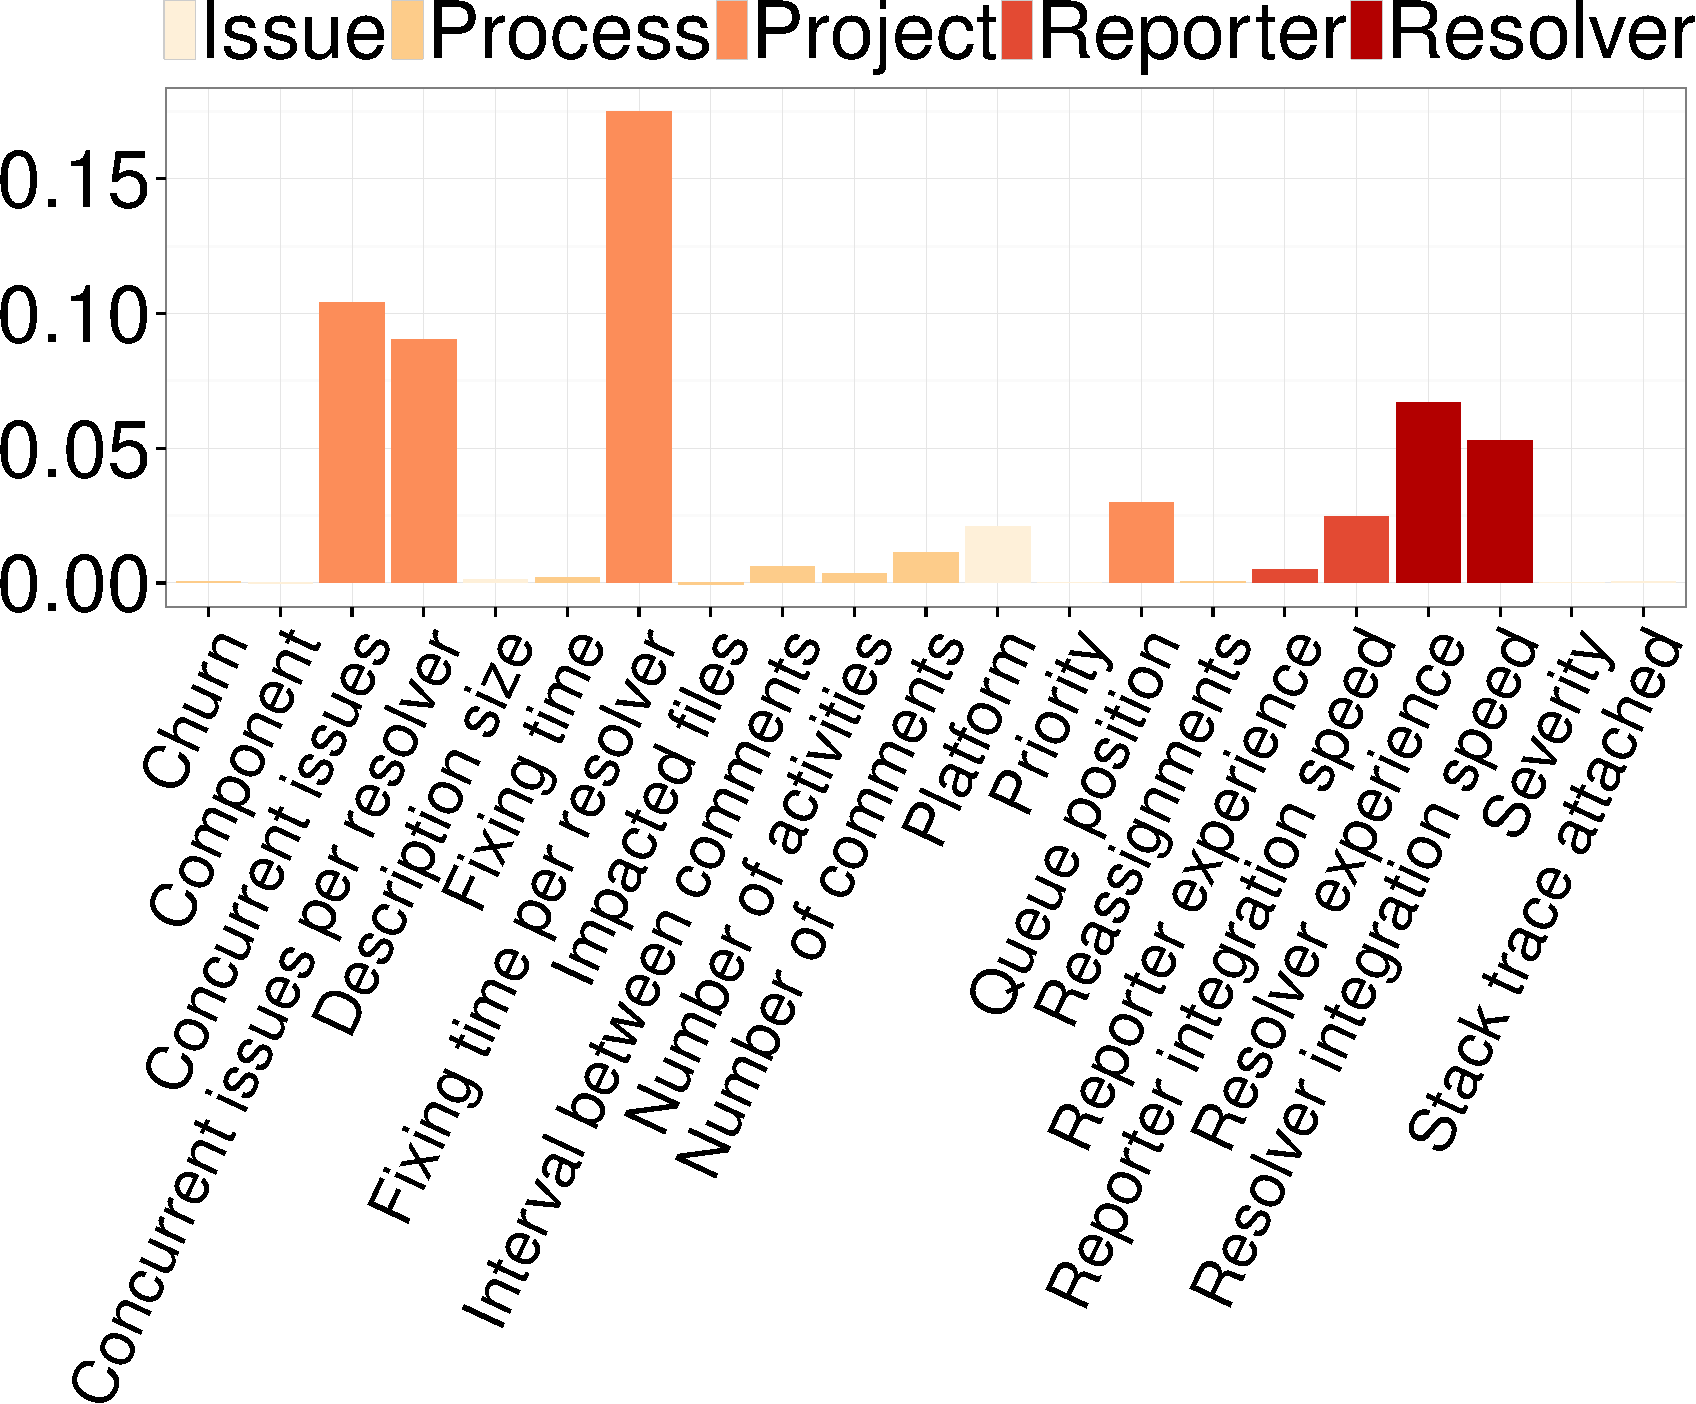
\includegraphics[width=0.55\textwidth,keepaspectratio] 
		{chapters/chapter4/figures/eclipse_loocv_varimp.pdf}
	\label{ch4:fig:impEclipse}
	}

	\subfloat[Firefox]{
		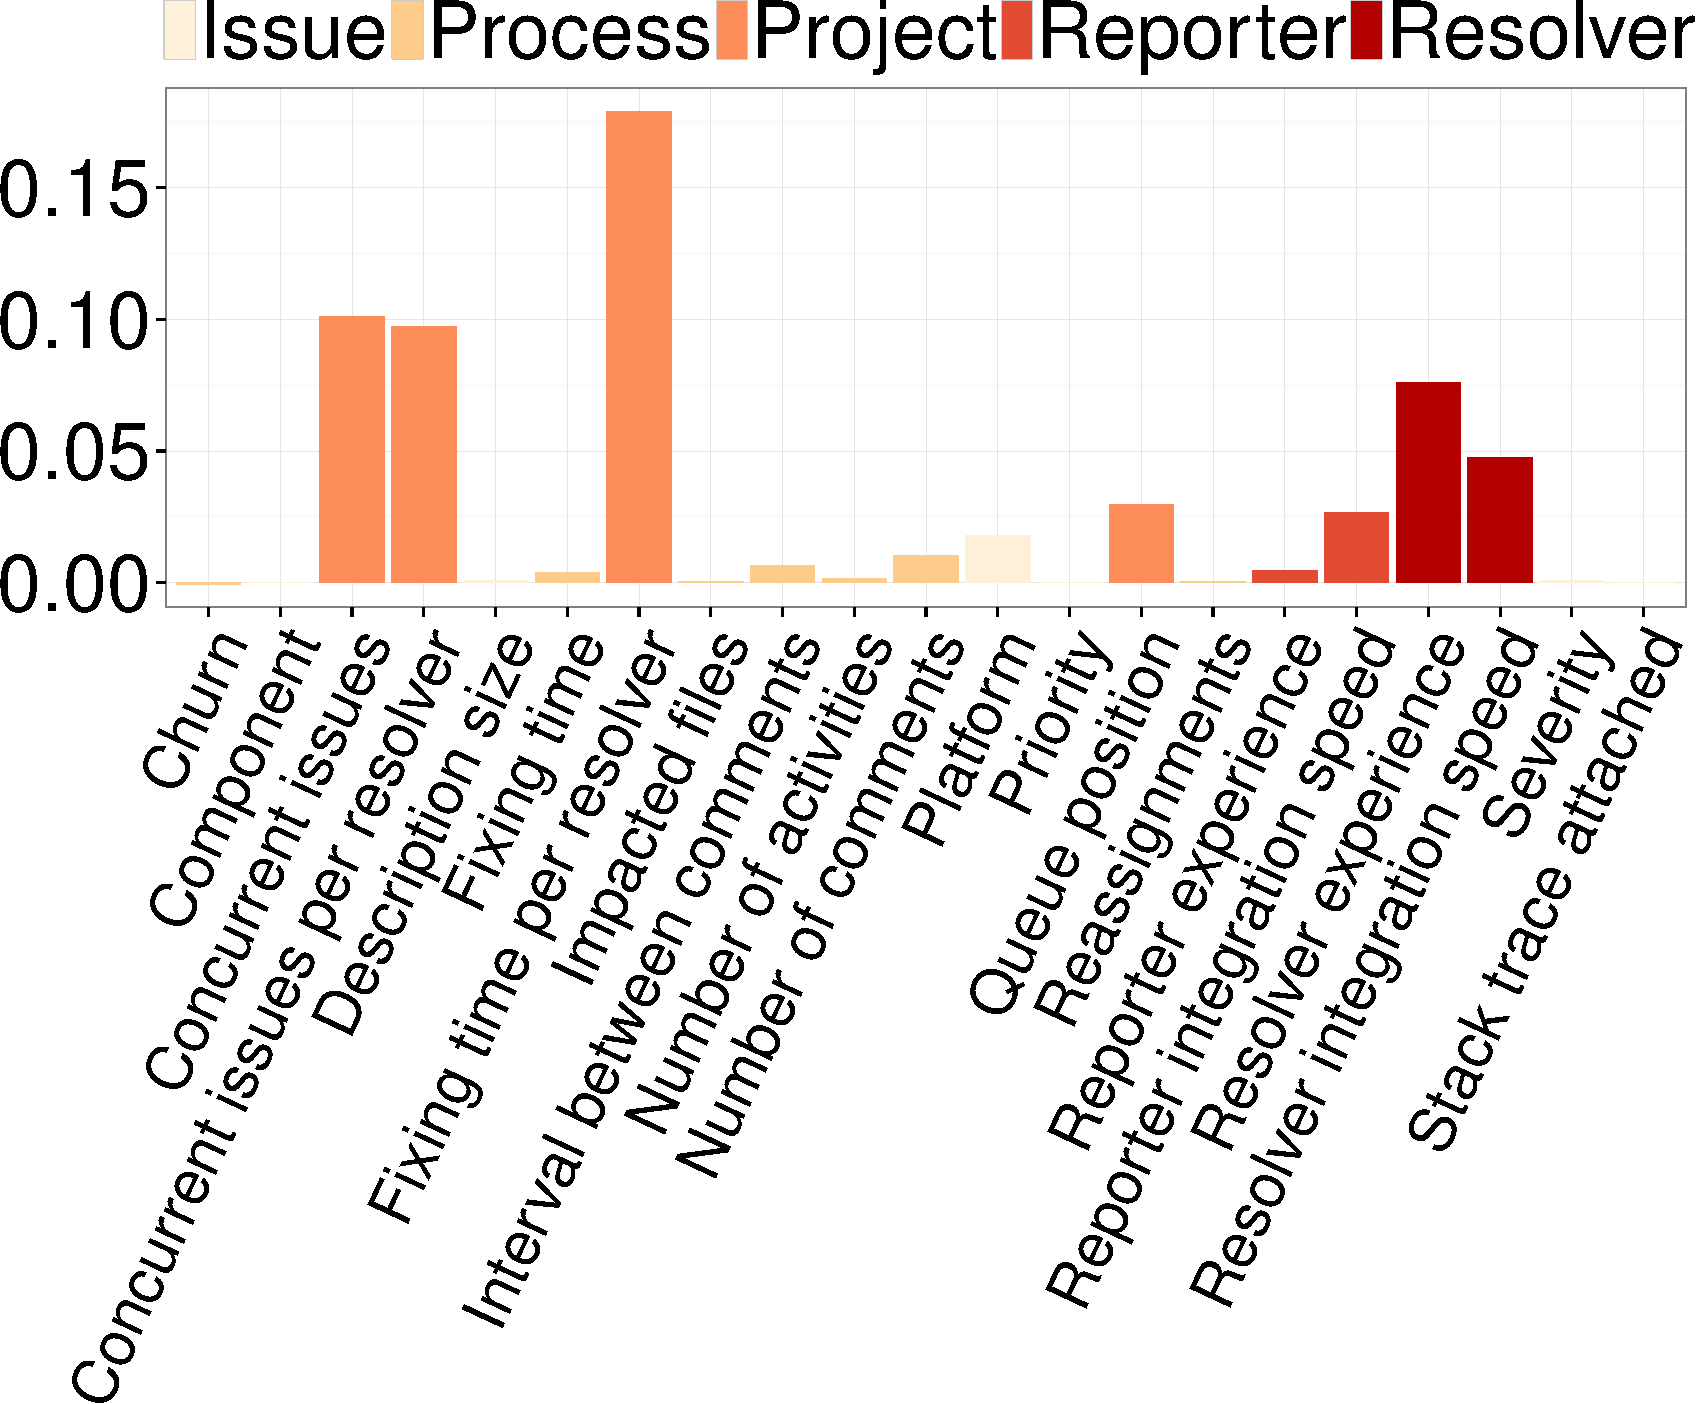
\includegraphics[width=0.55\textwidth,keepaspectratio]  
		{chapters/chapter4/figures/firefox_loocv_varimp.pdf}
		\label{ch4:fig:impFirefox}
	}

	\subfloat[ArgoUML]{
		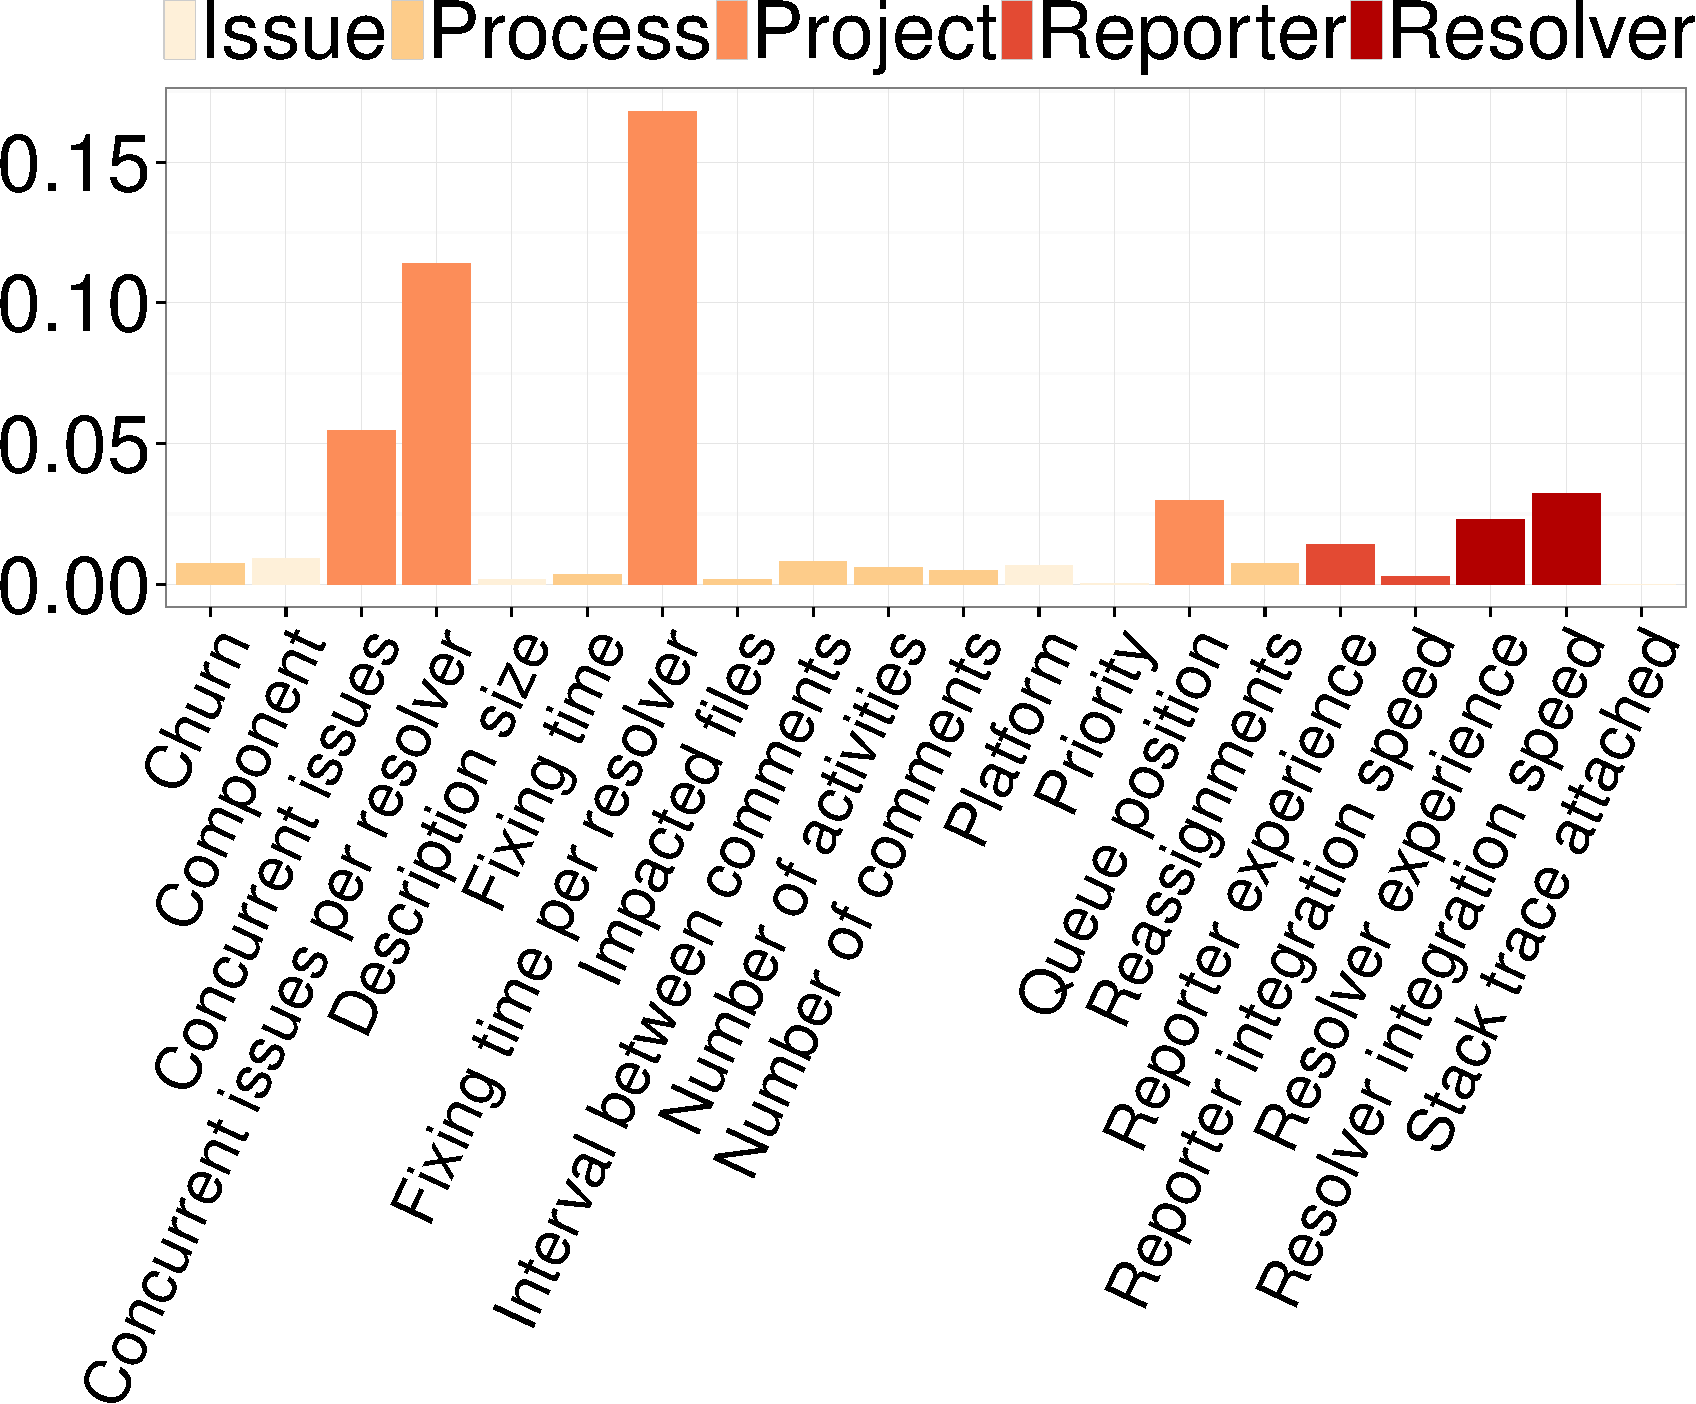
\includegraphics[width=0.55\textwidth,keepaspectratio] 
		{chapters/chapter4/figures/argouml_loocv_varimp.pdf}
	\label{ch4:fig:impArgo}}
	\caption{\textbf{Variable importance scores.} We show the 
		importance scores that are computed for the LOOCV of our models.}
	\label{ch4:fig:variableImportance}
\end{figure}

Our results suggest that the time that is invested by the resolvers on fixing
issues have a strong association with delivery delay. This could be due to
resolvers fixing issues more carefully---which would lead to a smoother
integration of such issues---or issues that were less complex in overall (\eg a
shorter time was invested), which might simplify the integration process. A deeper
analysis of this attribute would be necessary to better understand the exact
reasons behind this relationship (\eg consulting the development team through
surveys and interviews). 

We also observe that integration workload attributes (\ie \textit{backlog of
issues} and \textit{backlog of issues per resolver}) are the second most
influential attributes in the three studied projects. This finding suggests that
the integration backlog introduces overhead that may lead to longer integration
time.

\begin{figure}[!t]
	\centering
	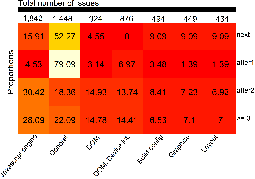
\includegraphics[width=0.60\textwidth,keepaspectratio]
	{chapters/chapter4/figures/firefox/RQ3_component_hm.pdf}
	\caption{\textbf{The spread of issues among the Firefox components.} The
		darker the colors, the smaller the proportion of issues that
	impact that component.}
	\label{ch4:fig:componentHeatmap}
\end{figure}

Furthermore, we study the distribution of addressed issues across components in the
Firefox project.
\hyperref[ch4:fig:componentHeatmap]{Figure}~\ref{ch4:fig:componentHeatmap} shows the top
seven components of the Firefox project, each having more than 400 addressed issues.
We analyze the proportion of addressed issues where integration was prevented in the
top seven components.
\hyperref[ch4:fig:componentHeatmap]{Figure}~\ref{ch4:fig:componentHeatmap} shows that,
for buckets \textit{next} and \textit{after-1}, the majority of issues are
related to the \textit{General component}, whereas for \textit{after-2} and
\textit{after-3-or-more} the majority are related to the \textit{Javascript
engine} component. Addressed issues related to the \textit{General} component
may be easy to integrate, whereas issues related to the \textit{Javascript
Engine} may require more careful analysis before integration.  \\


\noindent\textit{\textbf{Severity and priority have little influence on
delivery delay in terms of releases.}} Users and contributors of software
projects can denote the importance of an issue using the \textit{priority} and
\textit{severity} fields. Previous studies have shown that priority and
severity have little influence on bug fixing time
\cite{tian2015unreliability,Herraiz2008,Mockus:2002}. For example, while an
issue might be severe or of high priority, it might be complex and would take a
long time to fix.  

However, in the integration context, we expect that priority and severity would
be more influential, since the issues have already been addressed. Even though
priority and severity are often left at their default values (see
\hyperref[ch4:sec:subjects]{Section}~\ref{ch4:sec:subjects}), one would expect that the
integrators would fast-track the integration of issues for which they
care about increasing the levels of severity or priority. For instance,
according to the Eclipse project guidelines for filing issue reports, a priority
level of P1 is used for serious issues and specifies that the existence of a P1
issue should prevent a release from
shipping.\smartfoot{\url{http://wiki.eclipse.org/Development_Resources/HOWTO/Bugzilla_Use}}
Hence, it is surprising that priority and severity play such a small role in
determining the release in which an addressed issue will appear. Indeed,
\hyperref[ch4:fig:variableImportance]{Figure}~\ref{ch4:fig:variableImportance} shows
that the priority and severity metrics obtain low importance scores.

\begin{figure}
	\centering
	%\captionsetup{justification=centering}
	\subfloat[ArgoUML Priority]{
		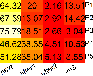
\includegraphics[width=0.30\textwidth,keepaspectratio] 
		{chapters/chapter4/figures/argouml/RQ3_priority_hm.pdf}
	\label{ch4:fig:heatMap_argo}}
	\subfloat[Eclipse Priority]{
		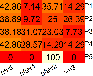
\includegraphics[width=0.30\textwidth,keepaspectratio] 
		{chapters/chapter4/figures/eclipse/RQ3_priority_hm.pdf}
	\label{ch4:fig:heatMap_eclipsep}}
	\subfloat[Firefox Priority]{
		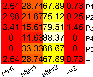
\includegraphics[width=0.30\textwidth,keepaspectratio]  
		{chapters/chapter4/figures/firefox/RQ3_priority_hm.pdf}
		\label{ch4:fig:heatMap_firefoxp}
	}

	\subfloat[Eclipse Severity]{
		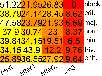
\includegraphics[width=0.35\textwidth,keepaspectratio] 
		{chapters/chapter4/figures/eclipse/RQ3_severity_hm.pdf}
	\label{ch4:fig:heatMap_eclipses}}
	\subfloat[Firefox Severity]{
		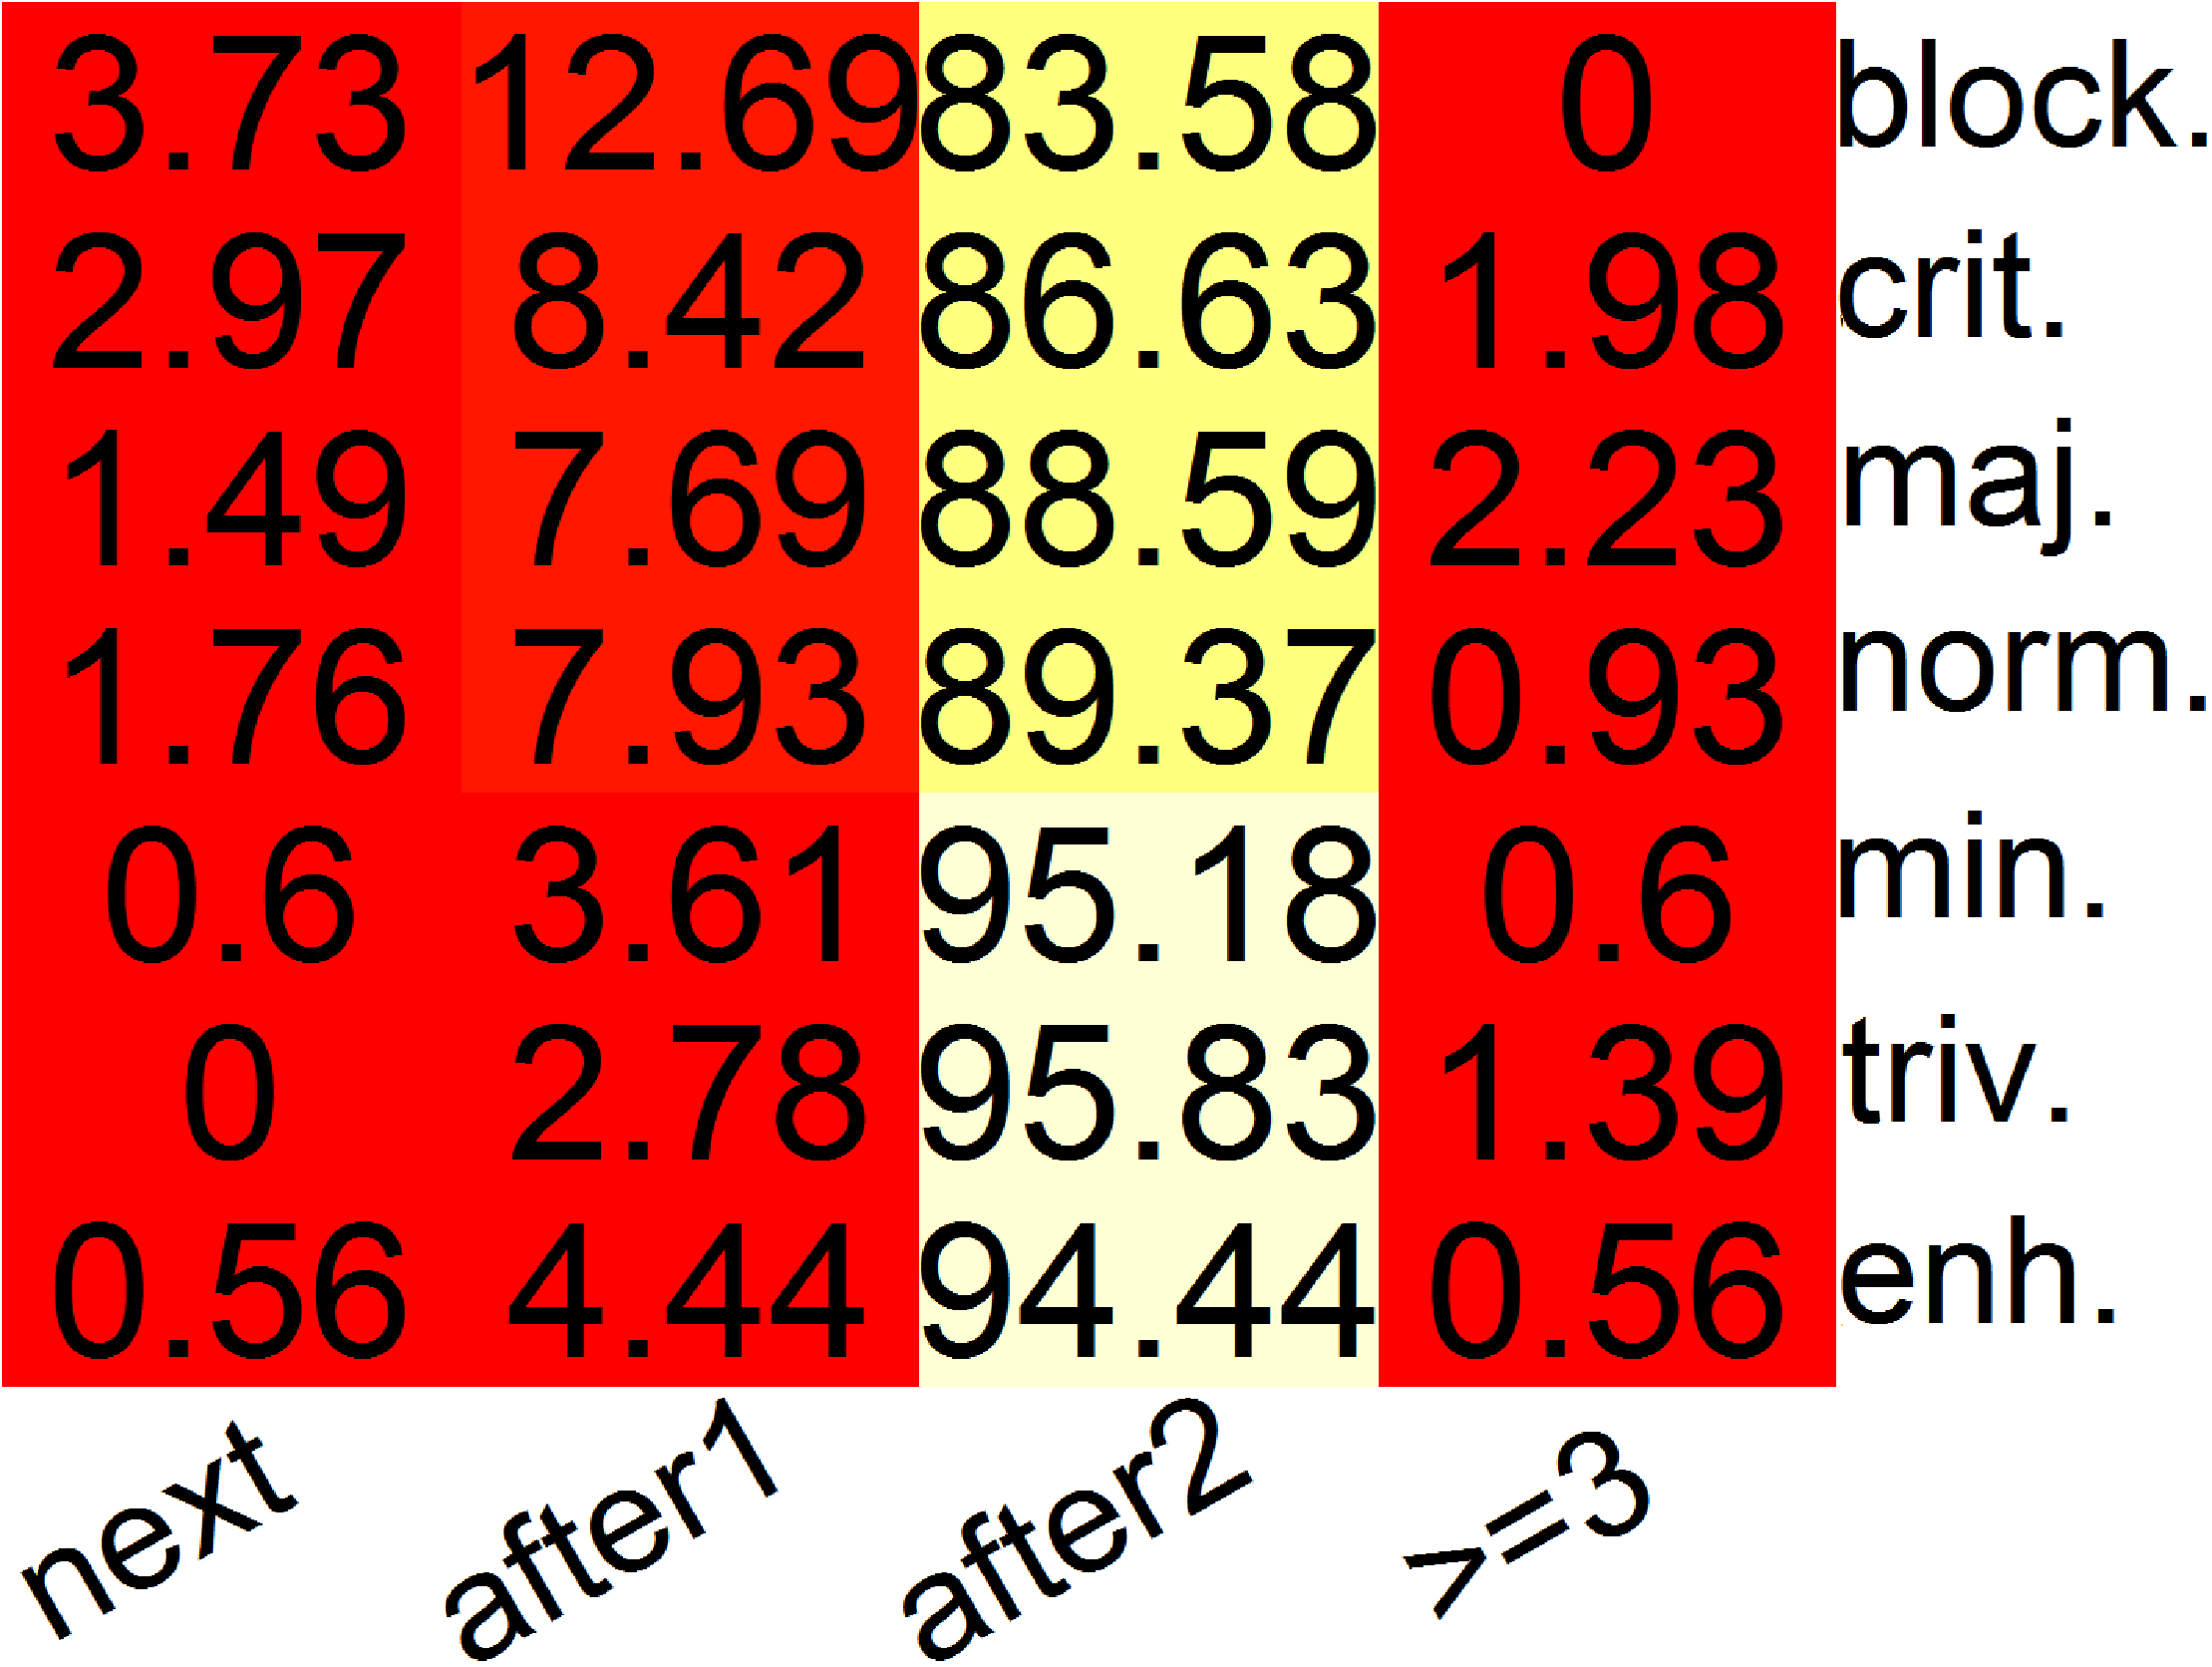
\includegraphics[width=0.35\textwidth,keepaspectratio]  
		{chapters/chapter4/figures/firefox/RQ3_severity_hm.pdf}
		\label{ch4:fig:heatMap_firefoxs}
	}
	\caption{\textbf{The percentage of priority and severity levels in each
		studied bucket of delivery delay.} We expect to see light
		colour in the upper left corner of these graphs, indicating that
		high priority/severity issues are integrated rapidly.
	Surprisingly, we are not seeing such a pattern in our datasets.}
	\label{ch4:fig:heatMaps}
\end{figure}

\hyperref[ch4:fig:heatMaps]{Figure}~\ref{ch4:fig:heatMaps} shows the percentage of
issues with a given priority (\textit{y-axis}) in a given integration bucket
(\textit{x-axis}). The integration of 36\% to 97\% of priority P1 addressed issues
had their integration prevented in at least one release, whereas the integration
of 32\% to 96\% of priority P2 addressed issues were prevented from integration in
at least one release. 

In the ArgoUML project, while the majority of priority P1 issues (64\%) were
integrated in the \textit{next} release, 36\% of them had their integration
prevented in at least one release. For the Firefox project, 97\% of the P1
issues and 96\% of the \textit{blocker} issues were prevented from integration
in at least one release. Finally, for the Eclipse project, 57\% of P1 issues and
49\% of blocker issues had their integration prevented in at least one release.
Hence, our data shows that, in the context of issue integration, the
\textit{priority} and \textit{severity} values that are recorded in the ITSs
have little influence on delivery delay. Instead, addressed issues might be
prioritized by the level of risk that are associated to
them.\smartfoot{Two issues from our sample were
	promoted to stabler release channels due to low associated risk \url{https://bugzilla.mozilla.org/show_bug.cgi?id=724145} and
\url{https://bugzilla.mozilla.org/show_bug.cgi?id=732962}, while another issue was prevented from integration due to code break
\url{https://bugzilla.mozilla.org/show_bug.cgi?id=723793}.} This might explain
why the time that is invested on fixing issues during a release cycle reduces
delivery delay---a risk of an addressed issue breaking the code would be
smaller when more time is invested at fixing activities. 

\conclusionbox{The total time that is invested in fixing issues of a release
	cycle and integration workload attributes are the most influential
	attributes in our models. We also find that priority and severity have
	little influence in estimating delivery delay.}

\subsubsection*{\textbf{\textit{RQ4: Results for delivery delay in terms of days}}}

\begin{table}[t]
	\scriptsize
	\centering
	\caption{\textbf{Explanatory power of attributes.} We present the
		$\chi^2$ proportion and the degrees of freedom that are spent
		for each attribute. The $\chi^2$ of the two most influential
		attributes of each model are in bold.
	\label{ch4:tbl:explanatory_power}}
	\begin{threeparttable}
		\begin{tabular}{llrrr}
			\cline{3-5} 
			\multicolumn{2}{c}{} & 
			Eclipse &
			Firefox &
			ArgoUML
			\tabularnewline
			\hline
			\multicolumn{2}{l}{Wald $\chi^2$} & 
			$1,180$ &
			$8,560$ &
			$2,803$
			\tabularnewline
			\hline 
			\multicolumn{2}{l}{Budgeted Degrees of Freedom} &
			$87$ & 
			$879$ &
			$102$
			\tabularnewline
			\hline
			\multicolumn{2}{l}{Degrees of Freedom Spent} &
			$24$ & 
			$33$ &
			$28$
			\tabularnewline
			\hline 
			\multirow{2}{*}{Reporter experience} & 
			D.F. & 
			$1$ & 
			$1$ &
			$1$
			\tabularnewline 
			& 
			$\chi^2$ & 
			$4^{\ast\ast\ast}$ &  
			$\approx 0$ &
			$1^{\ast\ast}$
			\tabularnewline
			\hline 
			\multirow{2}{*}{Resolver experience} & 
			D.F. & 
			$1$ & 
			$1$ &
			$1$
			\tabularnewline 
			& 
			$\chi^2$ & 
			$12^{\ast\ast\ast}$ & 
			$\approx 0^{\ast}$ &  
			$\approx 0$ 
			\tabularnewline
			\hline 
			\multirow{2}{*}{Reporter integration speed} & 
			D.F. & 
			$3$ & 
			$1$ &
			$2$
			\tabularnewline &
			$\chi^2$ & 
			$16^{\ast\ast\ast}$ &
			$\approx 0$ &
			$1^{\ast}$
			\tabularnewline  
			\hline 
			\multirow{2}{*}{Resolver integration speed} & 
			D.F. & 
			$2$ & 
			$1$ &
			$4$
			\tabularnewline & 
			$\chi^2$ & 
			$\mathbf{22}^{\ast\ast\ast}$ &
			$\approx 0$ &  
			$\mathbf{9}^{\ast\ast\ast}$
			\tabularnewline
			\hline 
			\multirow{2}{*}{Fixing time} & 
			D.F. & 
			$2$ & 
			\multirow{2}{*}{$\oplus$} &
			$1$
			\tabularnewline & 
			$\chi^2$ & 
			$1^{\ast}$ &
			&  
			$1^{\ast\ast}$ 
			\tabularnewline
			\hline 
			\multirow{2}{*}{Severity} & 
			D.F. & 
			$6$ &
			$6$ &
			\multirow{2}{*}{$\ominus$} 
			\tabularnewline & 
			$\chi^2$ &
			$\approx 0$ &
			$8^{\ast\ast\ast}$ &
			%\ominus
			\tabularnewline \hline 
			\multirow{2}{*}{Priority} &
			D.F. & 
			\multirow{2}{*}{$\oslash$} & 
			$5$ &
			$5$
			\tabularnewline & 
			$\chi^2$ & 
			&%\oslash
			$5^{\ast\ast\ast}$ &  
			$1^{\ast}$  
			\tabularnewline \hline 
			\multirow{2}{*}{Description size} & 
			D.F. & 
			$1$ & 
			$1$ &
			$1$
			\tabularnewline & 
			$\chi^2$ & 
			$\approx 0$ &  
			$\approx 0$ &
			$\approx 0$
			\tabularnewline \hline 
			\multirow{2}{*}{Impacted files} & 
			D.F. & 
			$1$ &
			$1$ &
			$1$
			\tabularnewline & 
			$\chi^2$ & 
			$\approx 0$ &
			$\approx 0^{\ast\ast}$ &
			$\approx $
			\tabularnewline \hline 
			\multirow{2}{*}{Number of comments} & 
			D.F. & 
			$1$ &
			$1$ &  
			$1$
			\tabularnewline & 
			$\chi^2$ & 
			$2^{\ast\ast}$ &  
			$1^{\ast\ast\ast}$  &
			$\approx 0$
			\tabularnewline \hline 
			\multirow{2}{*}{Reassignments} & 
			D.F. & 
			$1$ & 
			$1$ &
			$1$
			\tabularnewline & 
			$\chi^2$ & 
			$\approx 0$ &  
			$\approx 0$ &
			$1^{\ast}$
			\tabularnewline \hline 
			\multirow{2}{*}{Number of activities} & 
			D.F. & 
			$1$ &
			$1$ &
			$1$
			\tabularnewline & 
			$\chi^2$ & 
			$\approx 0$ &  
			$\approx 0$ &
			$\approx 0$
			\tabularnewline \hline 
			\multirow{2}{*}{Interval between comments} & 
			D.F. & 
			$1$ &
			$1$ &
			\multirow{2}{*}{$\oslash$}
			\tabularnewline & 
			$\chi^2$ & 
			$1^{\ast}$ &  
			$\approx 0$ &
			%\oslash correlation
			\tabularnewline \hline 
			\multirow{2}{*}{Churn} & 
			D.F. & 
			$1$ &
			$1$ &
			$1$
			\tabularnewline & 
			$\chi^2$ & 
			$\approx 0$ &  
			$\approx 0$ &
			$1^{\ast\ast}$
			\tabularnewline \hline 
			\multirow{2}{*}{Number of concurrent issues} & 
			D.F. & 
			\multirow{2}{*}{$\oslash$} &
			$2$ &
			\multirow{2}{*}{$\oslash$}
			\tabularnewline &
			$\chi^2$ &
			& %\oslash
			$\mathbf{8}^{\ast\ast\ast}$ &
			%\oslash
			\tabularnewline \hline 
			\multirow{2}{*}{Number of concurrent issues per resolver} & 
			D.F. & 
			$1$ & 
			$2$ &
			$2$
			\tabularnewline &
			$\chi^2$ &
			$7^{\ast\ast\ast}$ &  
			$2^{\ast\ast\ast}$ &
			$\mathbf{9}^{\ast\ast\ast}$
			\tabularnewline \hline 
			\multirow{2}{*}{Queue position} & 
			D.F. & 
			$1$ &             
			$4$ &
			$2$
			\tabularnewline & 
			$\chi^2$ & 
			$\mathbf{23}^{\ast\ast\ast}$ & 
			$\mathbf{83}^{\ast\ast\ast}$ &
			$\mathbf{67}^{\ast\ast\ast}$
			\tabularnewline \hline 
			\multirow{1}{*}{Fixing time per resolver} & 
			D.F. & 
			$1$ & 
			$2$ &
			$4$
			\tabularnewline &
			$\chi^2$ & 
			$7^{\ast\ast\ast}$ & 
			$\approx 0^{\ast\ast}$ &
			$8^{\ast\ast\ast}$
			\tabularnewline \hline 
		\end{tabular}
		\begin{tablenotes}
		\item[$\oslash$] Discarded during correlation analysis 
		\item[$\oplus$] Discarded during redundancy analysis 
		\item[$\ominus$] The variable does not apply to the dataset
		\item[$\ast$] $p < 0.05$
		\item[$\ast\ast$] $p < 0.01$
		\item[$\ast\ast\ast$] $p < 0.001$ 
		\end{tablenotes}
	\end{threeparttable}
\end{table}

\noindent\textbf{\textit{Project family attributes, such as the backlog of
issues and queue position provide most of the explanatory power of our models.}}
\hyperref[ch4:tbl:explanatory_power]{Table}~\ref{ch4:tbl:explanatory_power} shows the
explanatory power of each of the attributes of our models. The two most
influential attributes for each model are shown in bold. \textit{Queue
position}, \ie the time at which an issue is addressed is the most influential
attribute in all of the models that are fitted to our studied projects.
Interestingly, we observe that \textit{resolver integration speed}---the median
delivery delay of the previously resolved issues of a particular
resolver---plays an influential role in our models that are fit for the Eclipse
and ArgoUML projects. Moreover, we also observe that integration workload
attributes (\ie \textit{backlog of issues}, and \textit{backlog of issues per
resolver}) are very influential in our models that are fit for the Firefox and
ArgoUML projects.\\

\begin{figure}
	\centering
	\subfloat[Eclipse]{
		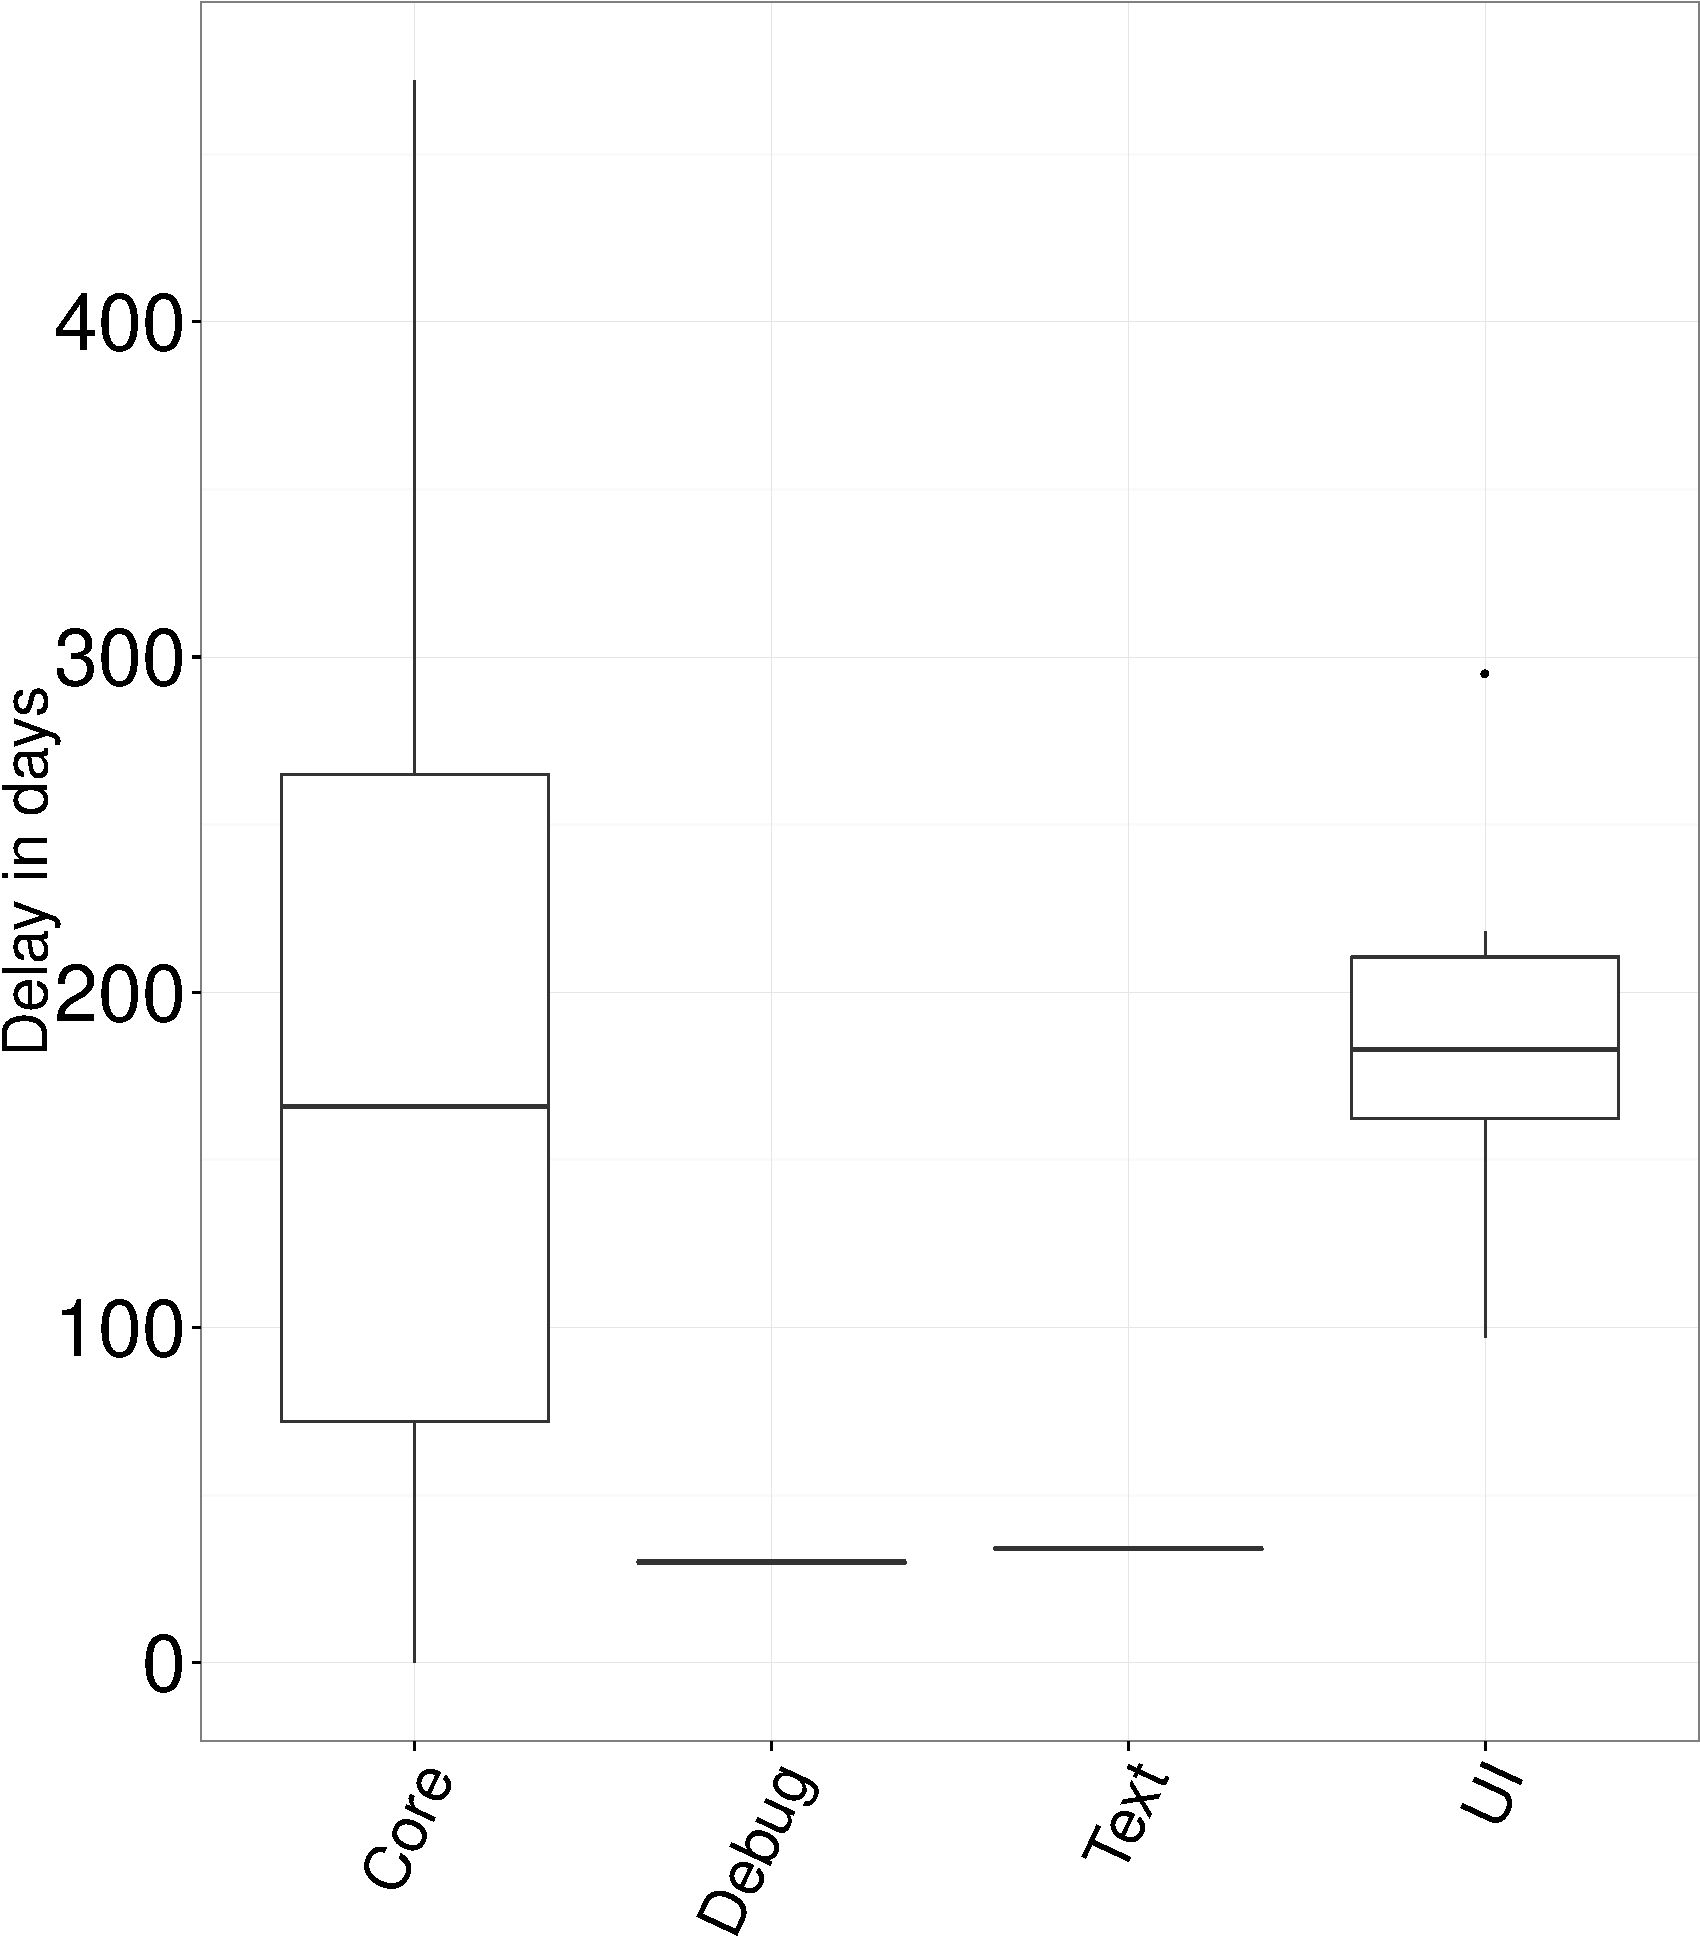
\includegraphics[width=0.40\textwidth,keepaspectratio]
		{chapters/chapter4/figures/components_eclipse.pdf}
	}

	\subfloat[Firefox]{
		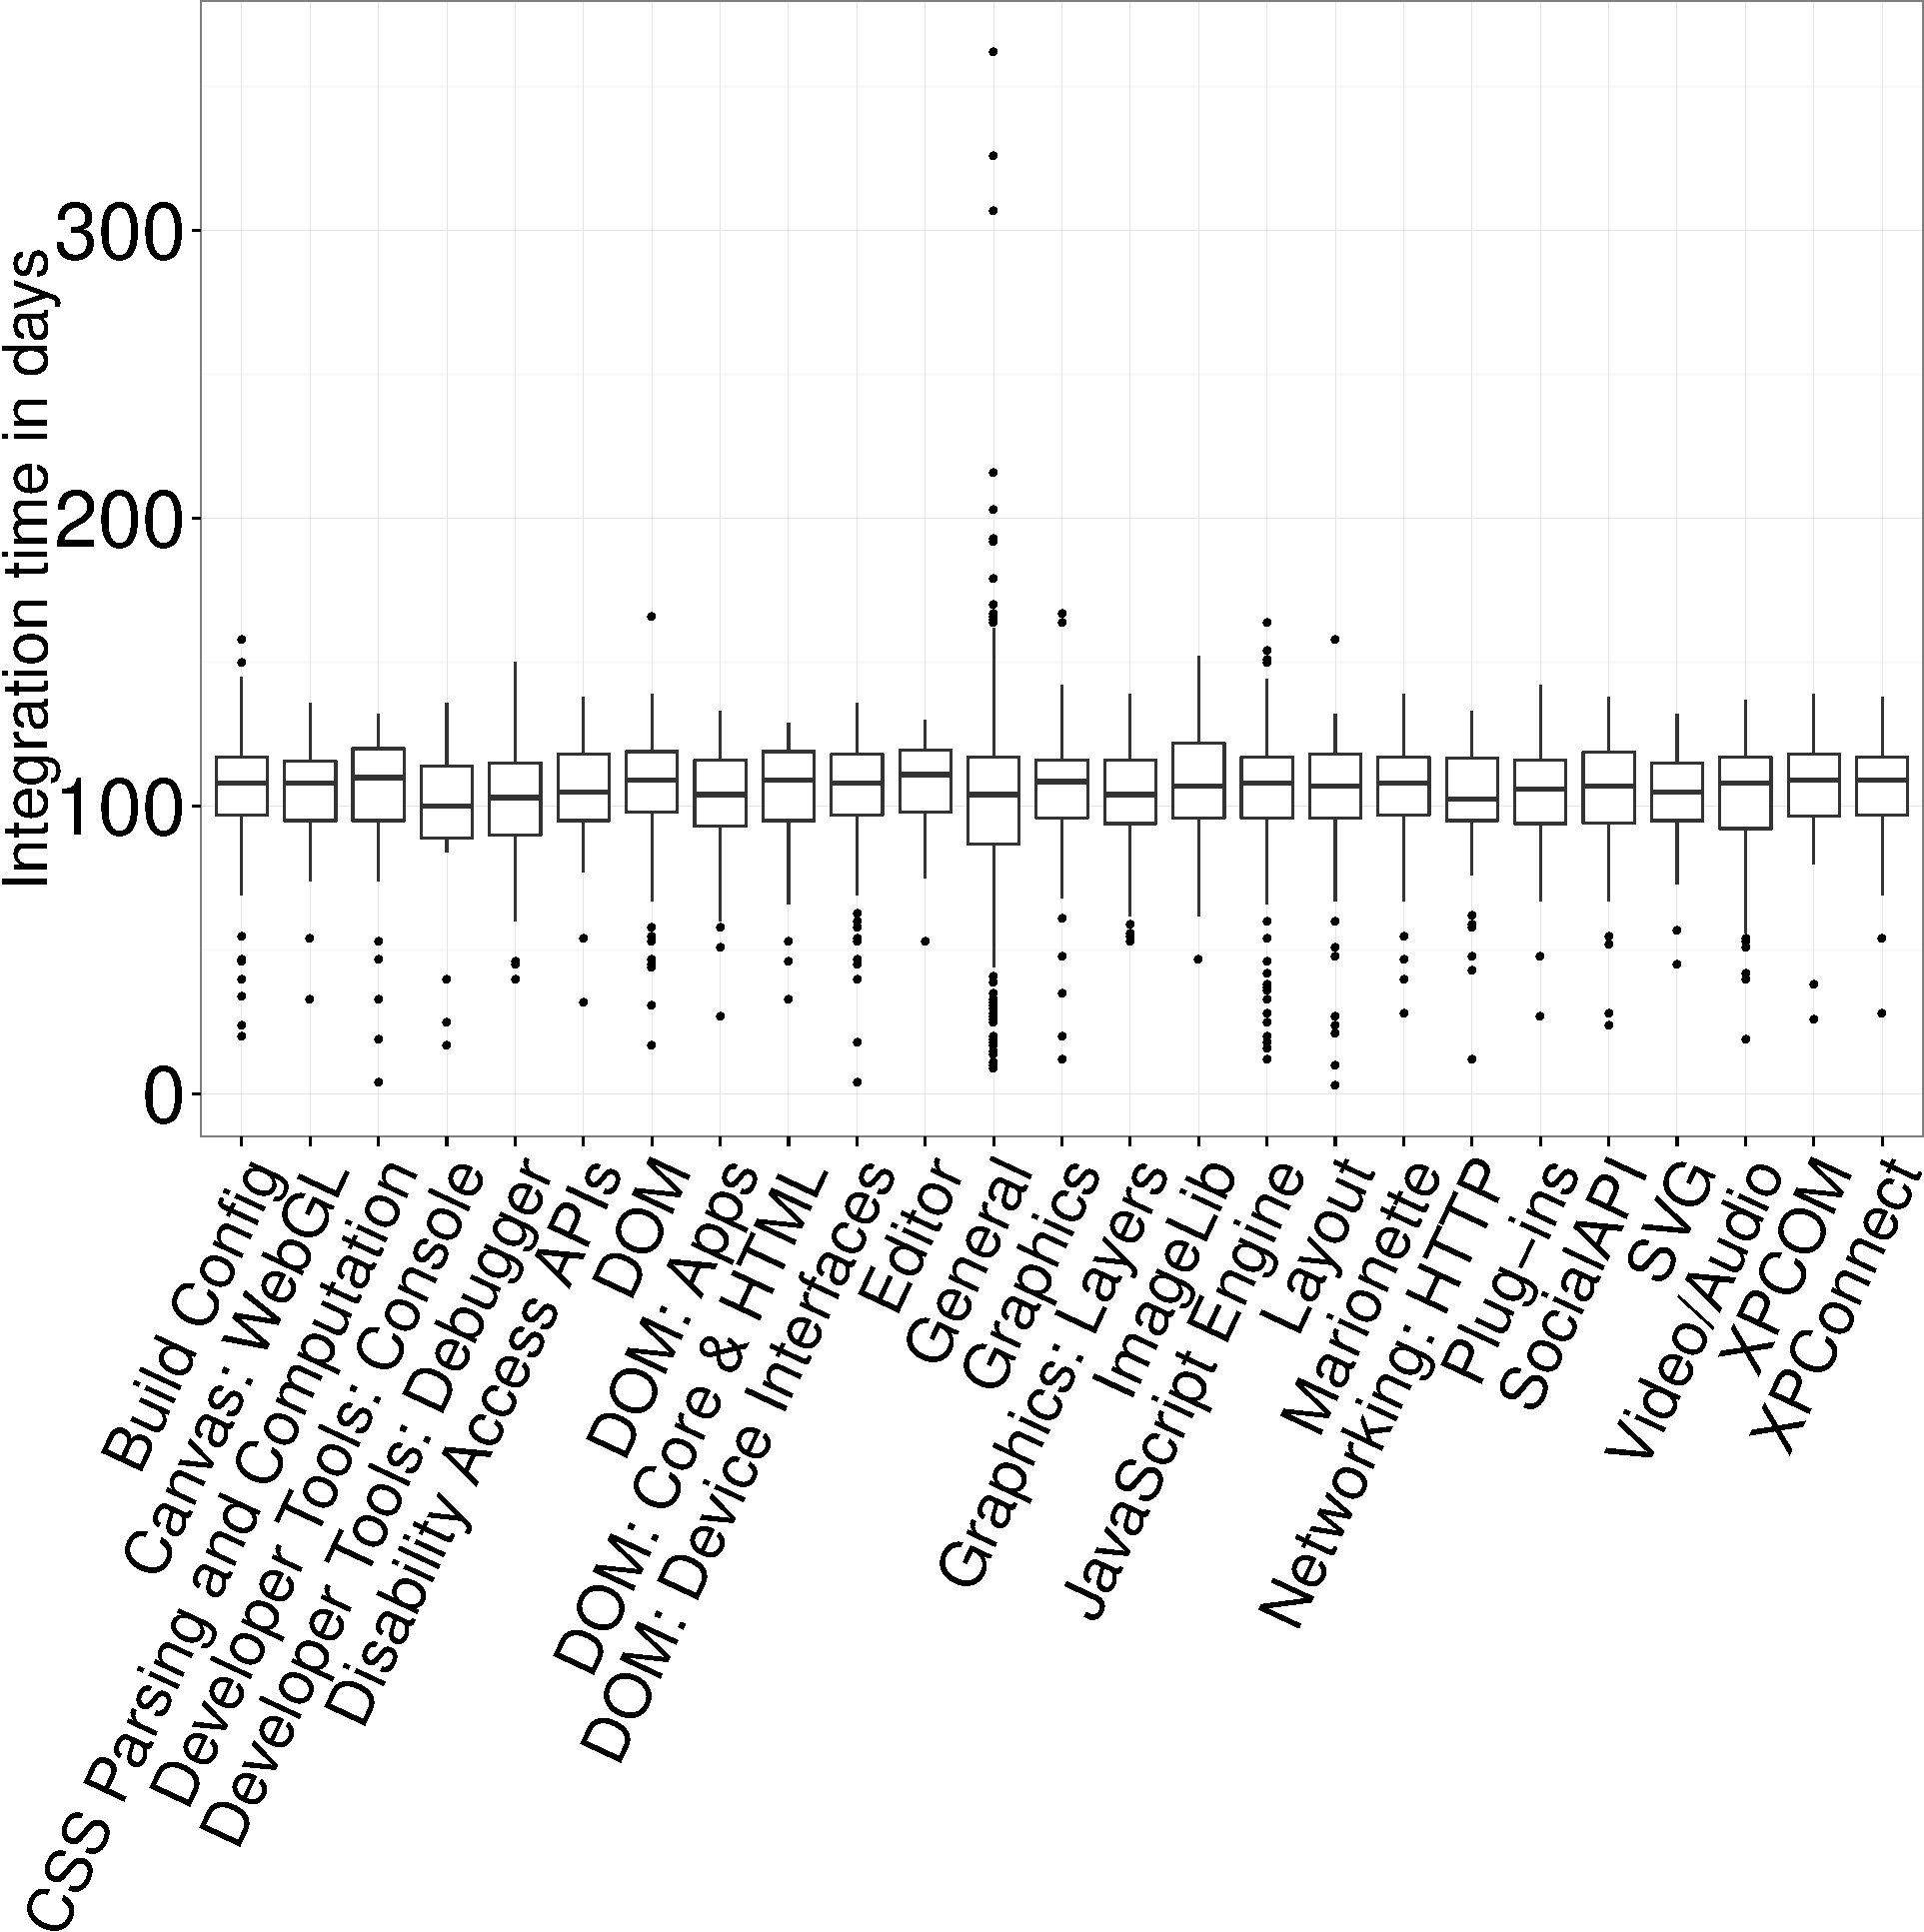
\includegraphics[width=0.40\textwidth,keepaspectratio]
		{chapters/chapter4/figures/components_firefox.pdf}
	}

	\subfloat[ArgoUML]{
		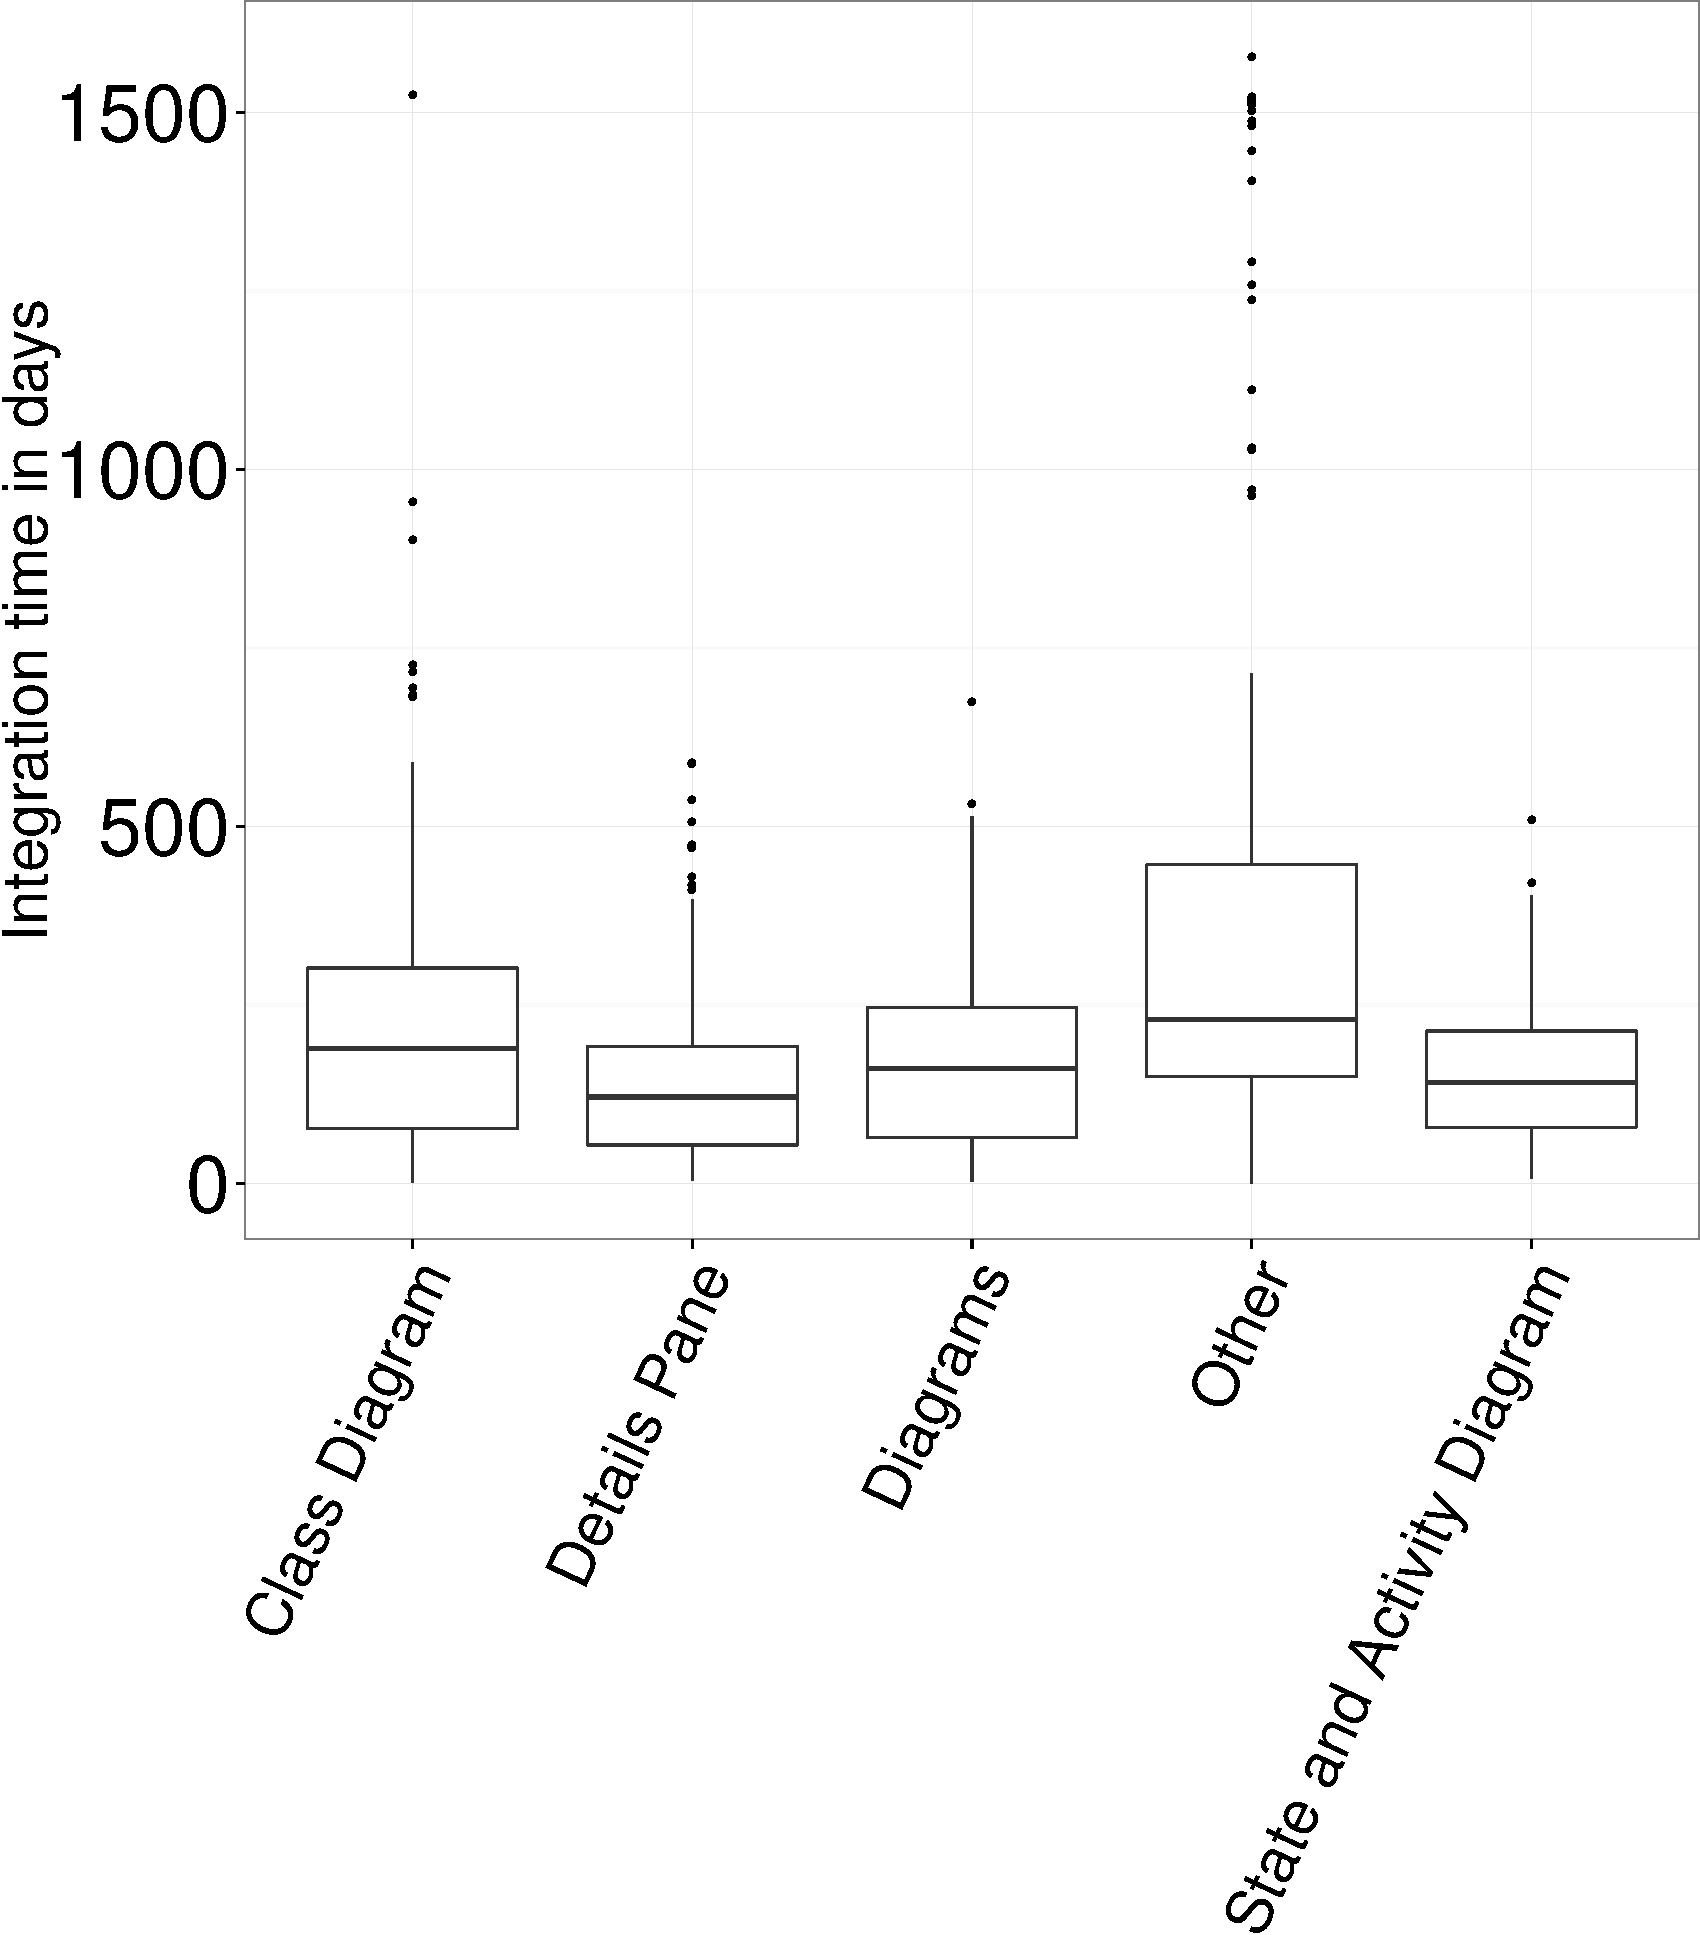
\includegraphics[width=0.40\textwidth,keepaspectratio]
		{chapters/chapter4/figures/components_argouml.pdf}
	}
	\caption{\textbf{Delivery delay per component.} The Figure shows the
		distributions of delivery delay in terms of days for each
		component of the studied projects.
	}
	\label{ch4:fig:component_analysis}
\end{figure}

\noindent\textbf{\textit{The component to which an issue is addressed has little
impact in the delivery delay in terms of days.}} To demonstrate this, we group
each addressed issue according to the components that such an issue modifies. We use
components that have at least 100 addressed issues as a threshold for our analysis.
We then compare the distribution of delivery delay in terms of days in these
components.
\hyperref[ch4:fig:component_analysis]{Figure}~\ref{ch4:fig:component_analysis} shows the
distributions of delivery delay in terms of days per component. We do not
observe a considerable difference between distributions of delivery delay in
the ArgoUML or Firefox projects. The distribution of the ``Other'' component in
the ArgoUML project is more skewed, which is suggestive of its generic
role---such a component may encompass a more broad spectrum of addressed issues. On
the other hand, 99\% of the addressed issues in the Eclipse (JDT) project belong to
the ``Core'' component (thus its skewness). Finally, the ``Debug'' and ``Text''
Eclipse components contain only one addressed issue each.   

\conclusionbox{The workload in terms of backlog of issues awaiting integration
	and the integration speed of prior addressed issues of a given resolver play
	a important role to model delivery delay in terms of days. Moreover,
	the initial \textit{queue position} is the most important attribute in
	all models that we fit to study delivery delay in terms of days.}



